


\chapter{Embedded System on Arm Cortex M4/M3}
\label{chap:arm_cortex}

\section{Introduction}

In this chapter, we study the ARM cortex M family processor. The reason behind studying this family of processors is because it is used in most microcontrollers. An example is shown in \autoref{fig:ARM_Cortex:example_arm_cortex_1}


\begin{figure}[h]
\centering
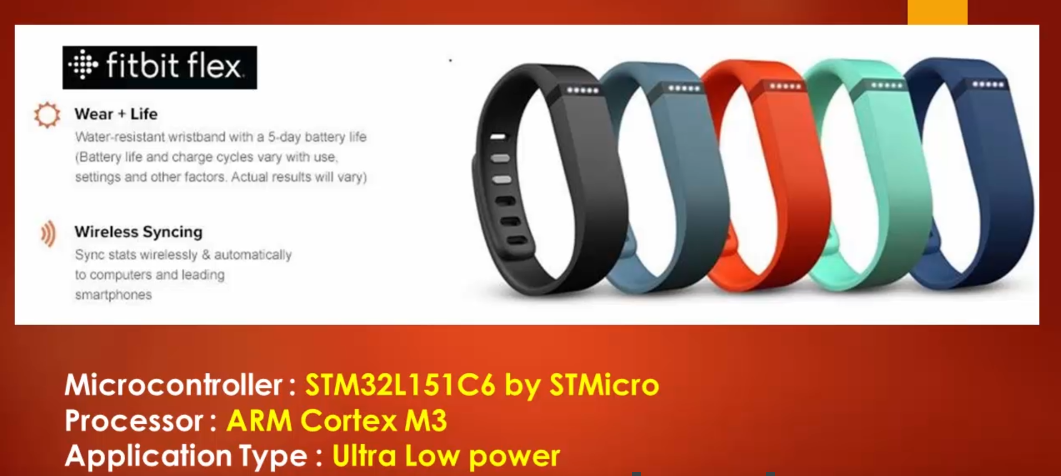
\includegraphics[scale=0.55]{Figures/ARM_Cortex/example_arm_cortex_1}
\caption{Example of ARM cortex used in industry}
\label{fig:ARM_Cortex:example_arm_cortex_1}
\end{figure}

The other usage of this processor can be find in \autoref{Chap:Arm_cortex:Summary}.\\

The major competitor for the ARM cortex architecture, is the AVR processors, widely used in arduino board. The AVR processor is manufactured by Microship. Also MSP 430 microcontroller (manufactured by Texas instrument) uses its own processor architecture.

\newpage
\subsection{Processor Core Vs Processor}

The best way to see the difference is via the ARM technical reference manual.\\


The cortex M4 block diagram is shown in \autoref{fig:ARM_Cortex:ARM_Cortex_M4_block}.


\begin{figure}[h]
\centering
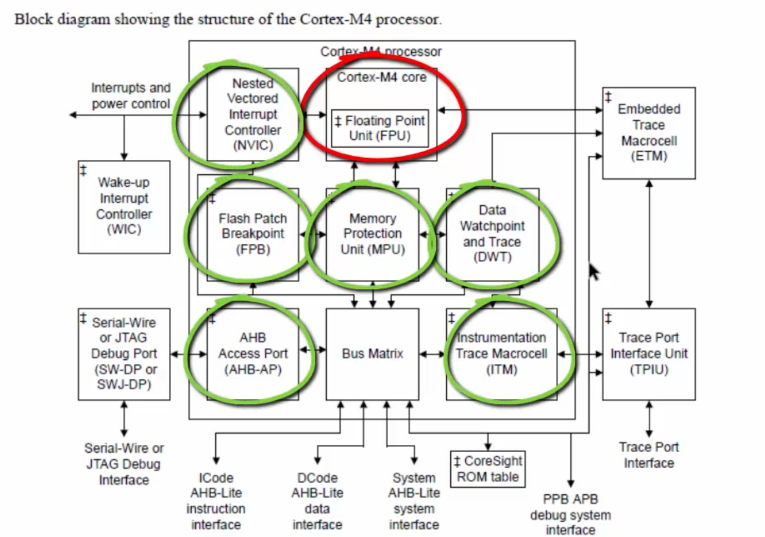
\includegraphics[scale=0.7]{Figures/ARM_Cortex/ARM_Cortex_M4_block}
\caption{AMR cortex M4 block diagram: Core + peripheral}
\label{fig:ARM_Cortex:ARM_Cortex_M4_block}
\end{figure}

\underline{Note:} \autoref{fig:ARM_Cortex:ARM_Cortex_M4_block} can be found in the Arm cortex M4 \tbi{technical reference manual}, section 2.1.\\

A processor is nothing but a processor core + surrounding peripheral.

Also a processor is called a CPU. Since we have a single core, the M4 processor is known as \textit{single core processor}.\\

\tbi{Now the fundamental question: what is inside the components of M4 core?} 

\begin{itemize}
    \item ALU to perform computation 

    \item Instruction decoder to decode instructions and fetches them from memory to verify if they are valid instructions or not

    \item Registers (and special function register to manipulate data)
    
\end{itemize}


Later in the chapter will see the details of some of the surrounding peripherals of the core (such as NVIC and the bus matrix).

Note that the processors uses several interfaces (IC code,DC code,$\cdots$) to communicate with the outside world

\newpage
\subsection{Processor vs Microcontroller}

Now this is a more easy part. Simply, microcontroller is composed from peripheral (timers,GPIO,$\cdots$) and a processor.\\

The processor (such as Arm M4 cortex) comes in a software IP package, and it is given to the microcontroller vendor (such as stm microeletronics,NXP,$\cdots$), and they implement the interface between their architecture and the processor.\\

\underline{Note:} some microcontroller vendors such as Texas instrument implement their own processor architecture, and integrate it in its microcontroller architecture.

\newpage
\section{Operations Modes of Cortex Processor}
\label{Sec:Operations_Modes}

Now starting from this section and after, we will study several features of the cortex M0/M3/M4 processor, which are shown in \autoref{fig:ARM_Cortex:ARM_Cortex_features}.

\begin{figure}[h]
\centering
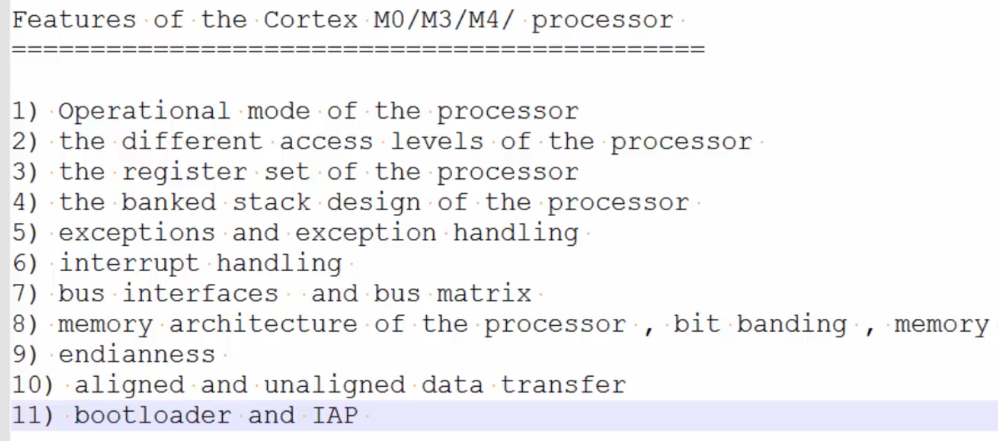
\includegraphics[scale=0.7]{Figures/ARM_Cortex/ARM_Cortex_features}
\caption{AMR cortex different features}
\label{fig:ARM_Cortex:ARM_Cortex_features}
\end{figure}

We start with the 1st point: operational mode of the processor.\\

\underline{Note:} this discussion will handle cortex family M0/M3/M4, but the general concepts can be applied to other families such as M8 family with some technical differences. In such case, we need to refer to the reference manual as always to cover the different details.\\

Now we start with general points concerning the operational mode, and then in the next section we implement some code to see these concepts. These general points are as follows:

\begin{itemize}
    \item The processor usually give us 2 mode: Thread mode (also known as user mode), and handler mode

    \item The processor always starts with thread mode, and all the application we code run under thread mode

    \item Whenever the processor meets some exception or interrupts coming from some peripheral,  the core will change its mode to handler mode, and interrupt will run under the handler mode
    
\end{itemize}

\newpage
\subsection{Operation Mode Demo}
\label{Sub:Operation_Mode_Demo}

\underline{Note:} See project \verb|operation-mode|

First we explain the general flow of the code

\begin{itemize}
    
    \item The code starts with thread mode by entering the \verb|main| function

    \begin{itemize}
        \item \underline{Note:} Before the \verb|main()|, there is function called \verb|reset-handler()| which will be called, then the \verb|main()| will be called later. But since we don't know the handler yet, we will skip it for now and takes the assumption that \verb|main()| function is executed first.
    \end{itemize}

    \item When the code enter \verb|generate-interrupt()|, it triggers an interrupt service using software, and the command \verb|*pSTIR = (3&0x1FF)| trigger the interrupt, implemented by the function \verb|void RTC-WKUP-IRQHandler(void)| 


    \item The function  \verb|void RTC-WKUP-IRQHandler(void)|  will switch the processor into handler mode

    \item Advantage of handler mode: we can access all resources of our microcontroller
    
\end{itemize}

Now how to know if the processor has switched from thread mode to handler mode ? This is done by status register called  \textit{interrupt program status register} (found in Table 2-5 from Arm cortex M4 generic user guide), shown in \autoref{fig:ARM_Cortex:ispr_bits}.

\begin{figure}[h]
\centering
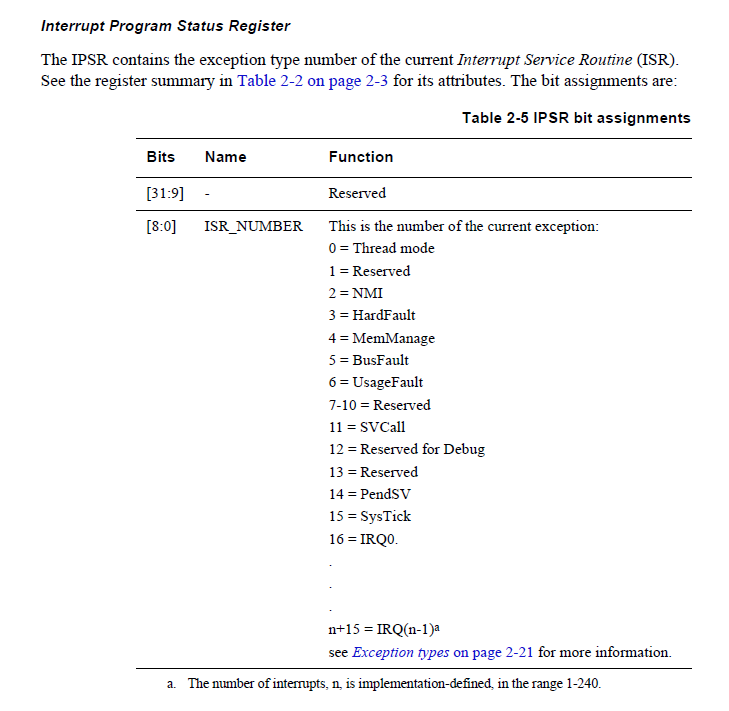
\includegraphics[scale=0.7]{Figures/ARM_Cortex/ispr_bits}
\caption{Interrupt program status register bit assignments}
\label{fig:ARM_Cortex:ispr_bits}
\end{figure}

By the running the code in a debug mode, the \verb|ispr| will have a value different from 0.

\newpage
\section{Access Levels}

Now we move to other technical term which is called \textit{access levels}. In a processor, we have 2 different type of access levels:

\begin{enumerate}
    \item Privilege access Level (PAL)

    \item Non-Privilege access Level (NPAL)
\end{enumerate}

In \autoref{fig:ARM_Cortex:summary_operation_access_level}, we have a summary block diagram which summarize the access levels along with operation mode (thread mode and handler mode)

\begin{figure}[h]
\centering
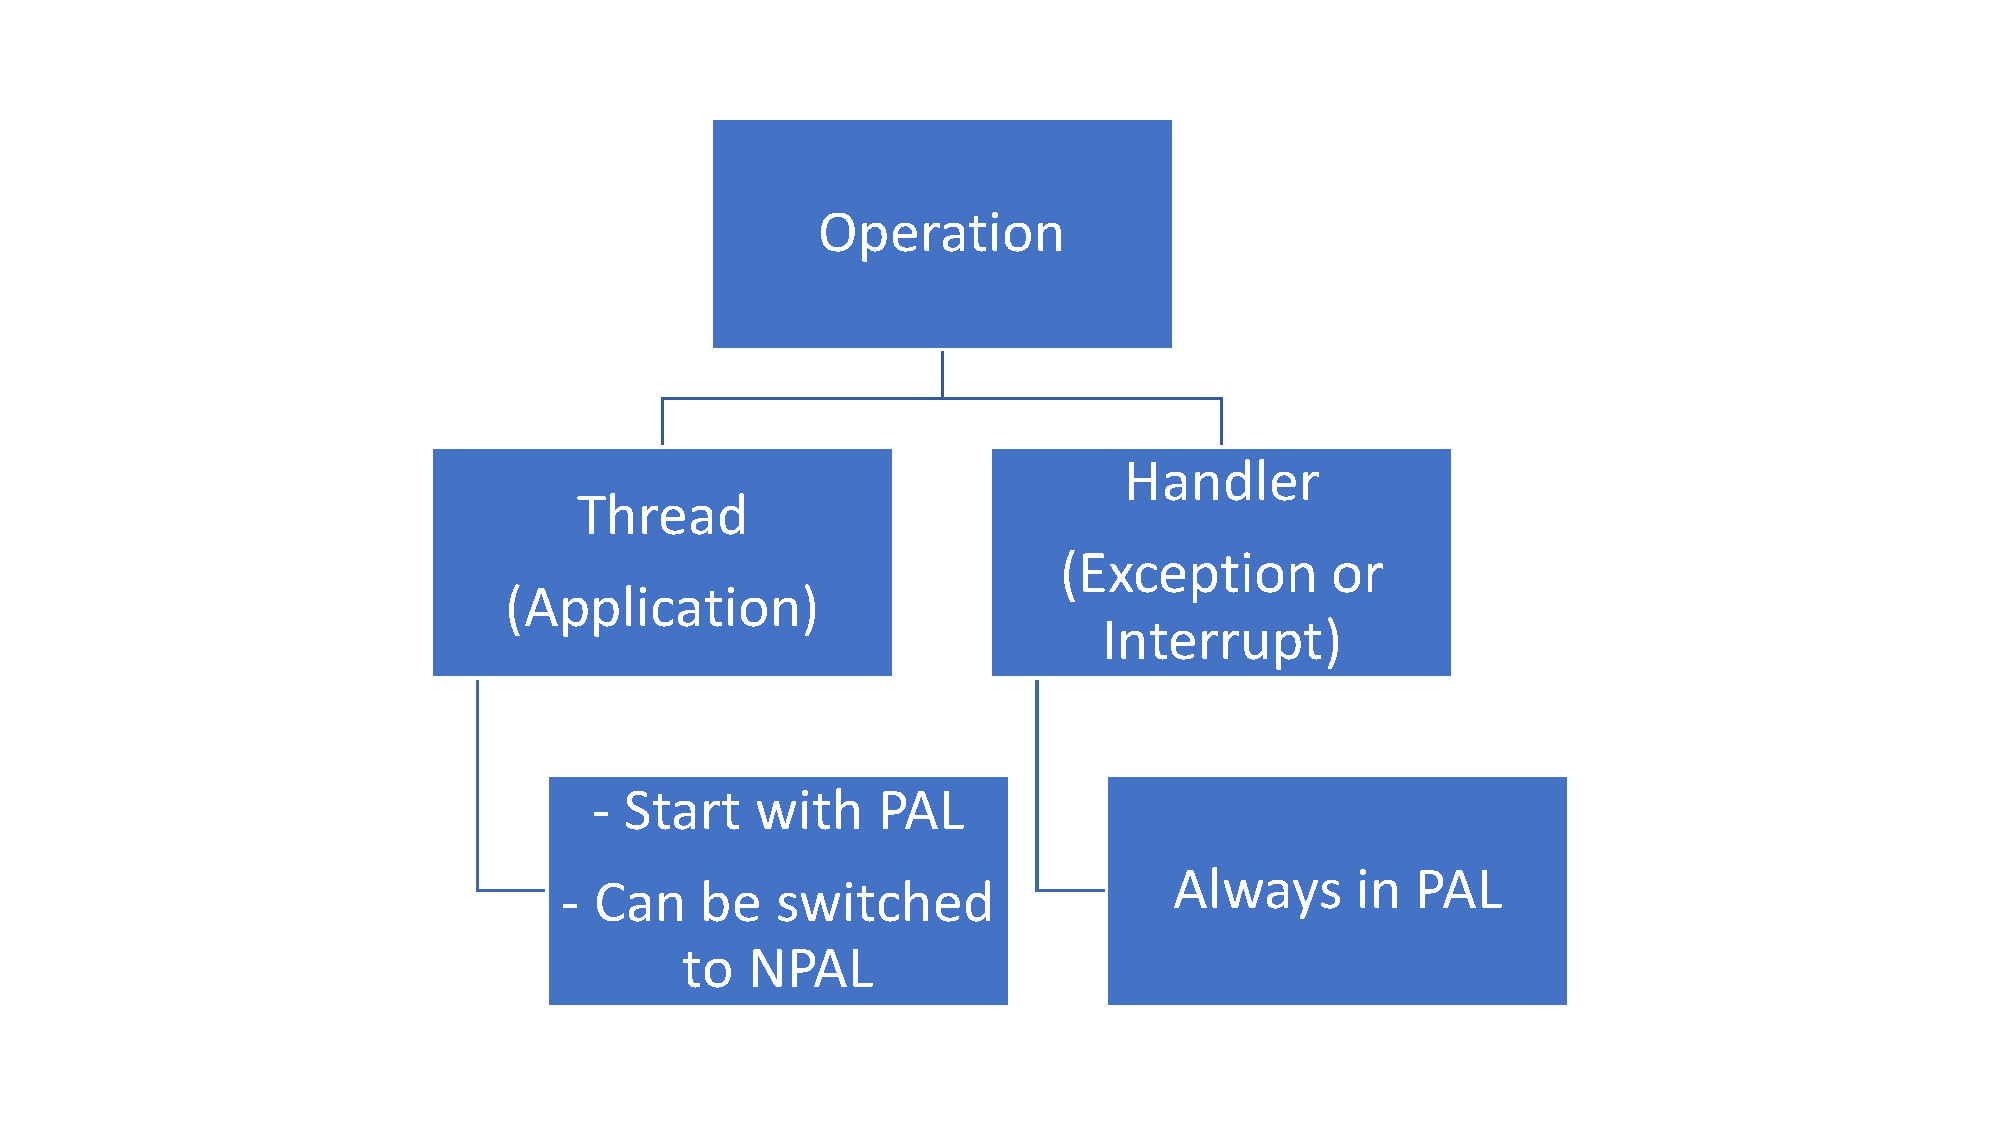
\includegraphics[scale=0.5]{Figures/ARM_Cortex/summary_operation_access_level}
\caption{Summary: Operation Mode and Access Level Mode}
\label{fig:ARM_Cortex:summary_operation_access_level}
\end{figure}

To switch between access levels of the processor, we need to configure the control register.

\newpage
\section{Core Registers}
\label{Sec:Core_Registers}

Core registers can be found in section 2.1.3 from the generic user guide of the cortex M4 processor. Its decomposition is also shown in \autoref{fig:ARM_Cortex:core_registers}.

\begin{figure}[h]
\centering
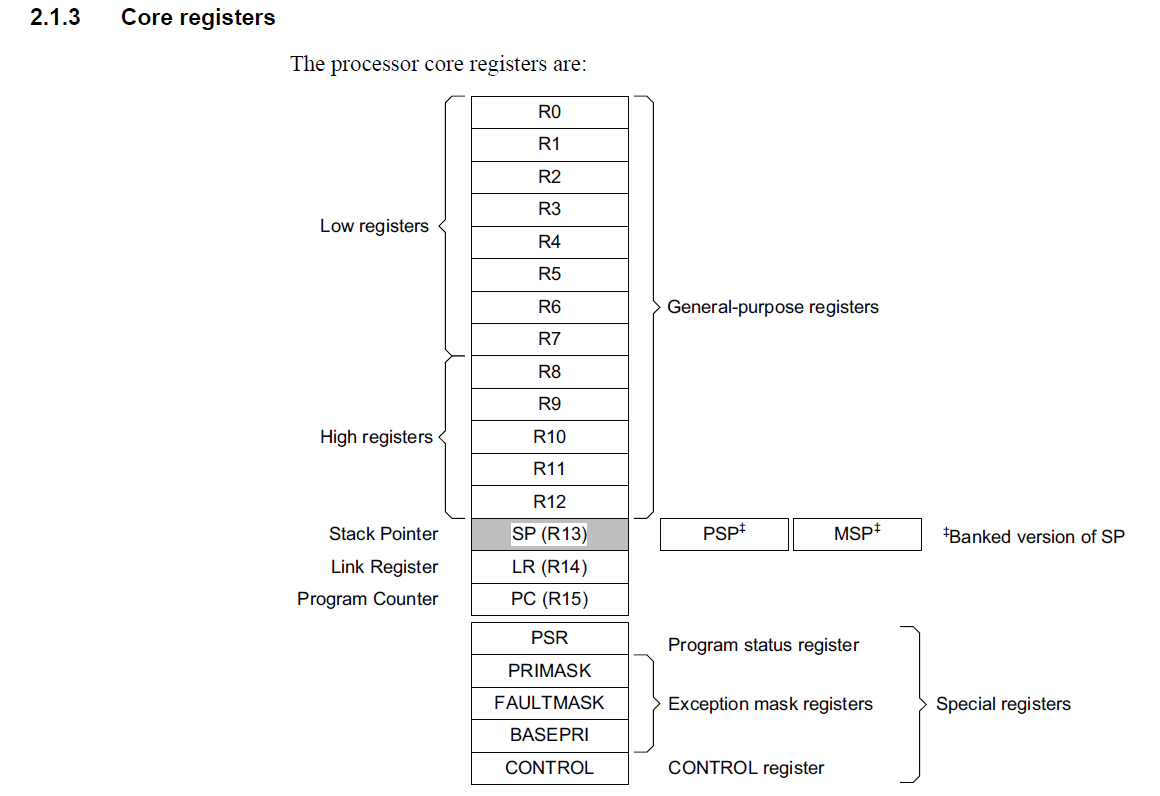
\includegraphics[scale=0.5]{Figures/ARM_Cortex/core_registers}
\caption{Summary: Operation Mode and Access Level Mode}
\label{fig:ARM_Cortex:core_registers}
\end{figure}

\begin{itemize}
    \item \verb|R0| $\rightarrow$ \verb|R12| (13 total registers) are general registers, used for example for data manipulation, data storage

    \item \verb|SP|: stack pointer register, which handle memory, and it can be used in 2 modes: PSP and MSP

    \item \verb|LR|: it stores the return address value from a function call, in order to return to the caller and continue the flow of the code. An example is shown in \autoref{fig:ARM_Cortex:core_registers_lr}.

\begin{figure}[h]
\centering
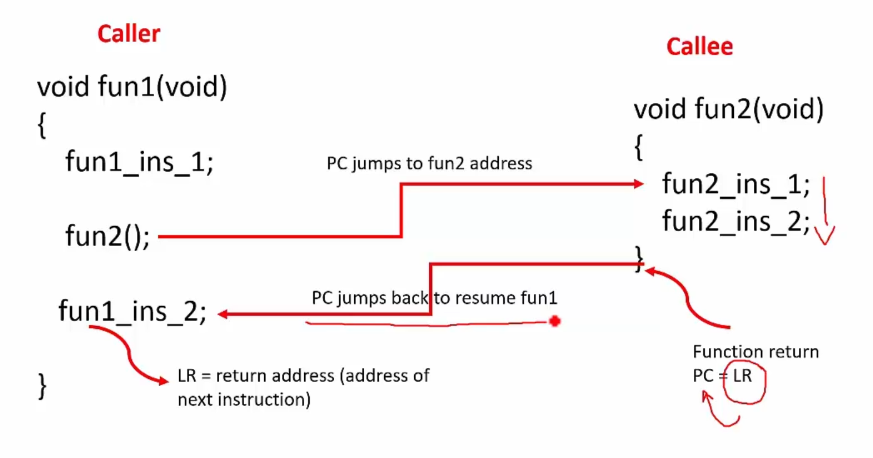
\includegraphics[scale=0.5]{Figures/ARM_Cortex/core_registers_lr}
\caption{LR register flow}
\label{fig:ARM_Cortex:core_registers_lr}
\end{figure}

    \todo{LR and assembly debugging} \underline{\textit{LR and assembly debugging}} : \textit{video 23 contains nice debugging in assembly mode. To redo it later}

    \item R15, the \verb|PC| register: holds the addressee of the next instruction to be executed

\newpage
    \item \verb|PSR|: is the combination of the 3 different register as shown in \autoref{fig:ARM_Cortex:psr_combination}

\begin{figure}[h]
\centering
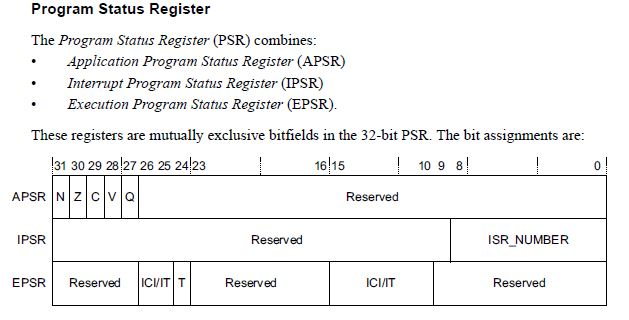
\includegraphics[scale=0.7]{Figures/ARM_Cortex/psr_combination}
\caption{PSR registers}
\label{fig:ARM_Cortex:psr_combination}
\end{figure}

    \begin{itemize}
        \item \verb|ASPR| for conditional flags (detect carry,overflow,$\cdots$)

        \item Other will be seen later during coding experiments
    \end{itemize}
    
\end{itemize}

\newpage
\section{Memory Mapped vs Non-Memory Mapped Registers}

In \autoref{Sec:Core_Registers}, we saw briefly different register relative to the core cortex M4. These registers are \tbi{non memory mapped}. Likewise, there exist some registers (relative to cortex processor, or for the MCU such as timers,GPIO,$\cdots$), which they are \tbi{memory mapped}, and we can access them using our \verb|C| code. \autoref{fig:ARM_Cortex:memory_and_nonmemory_mapped}  illustrates the differences between memory and non-memory mapped registers.

\begin{figure}[h]
\centering
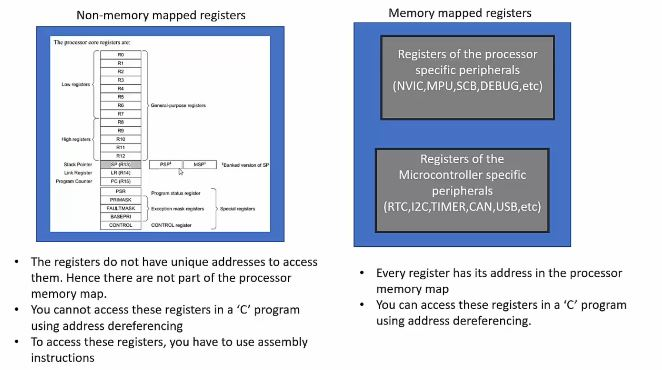
\includegraphics[scale=1.1]{Figures/ARM_Cortex/memory_and_nonmemory_mapped}
\caption{Memory vs Non-Memory mapped registers}
\label{fig:ARM_Cortex:memory_and_nonmemory_mapped}
\end{figure}


\newpage

\section{ARM GCC Inline Assembly}
\label{Sec:inline_assembly}

In this section we learn how to write inline assembly language. By inline we mean that the assembly language will be inside our \verb|C| program. The purpose behind this if we want to control some registers which are non memory mapped, and do some manipulation between the \verb|C| code and the arm cortex registers (example: move some result coming from a \verb|C| variable to some arm registers).\\


\underline{Note:} the syntax described in this section is only specific to ARM GCC compiler. Other compiler have different syntax.\\

\autoref{fig:ARM_Cortex:Inline_Assembly_example_syntax} contains example and the general syntax of arm assembly relative to ARM GCC compiler.

\begin{figure}[h]
\centering
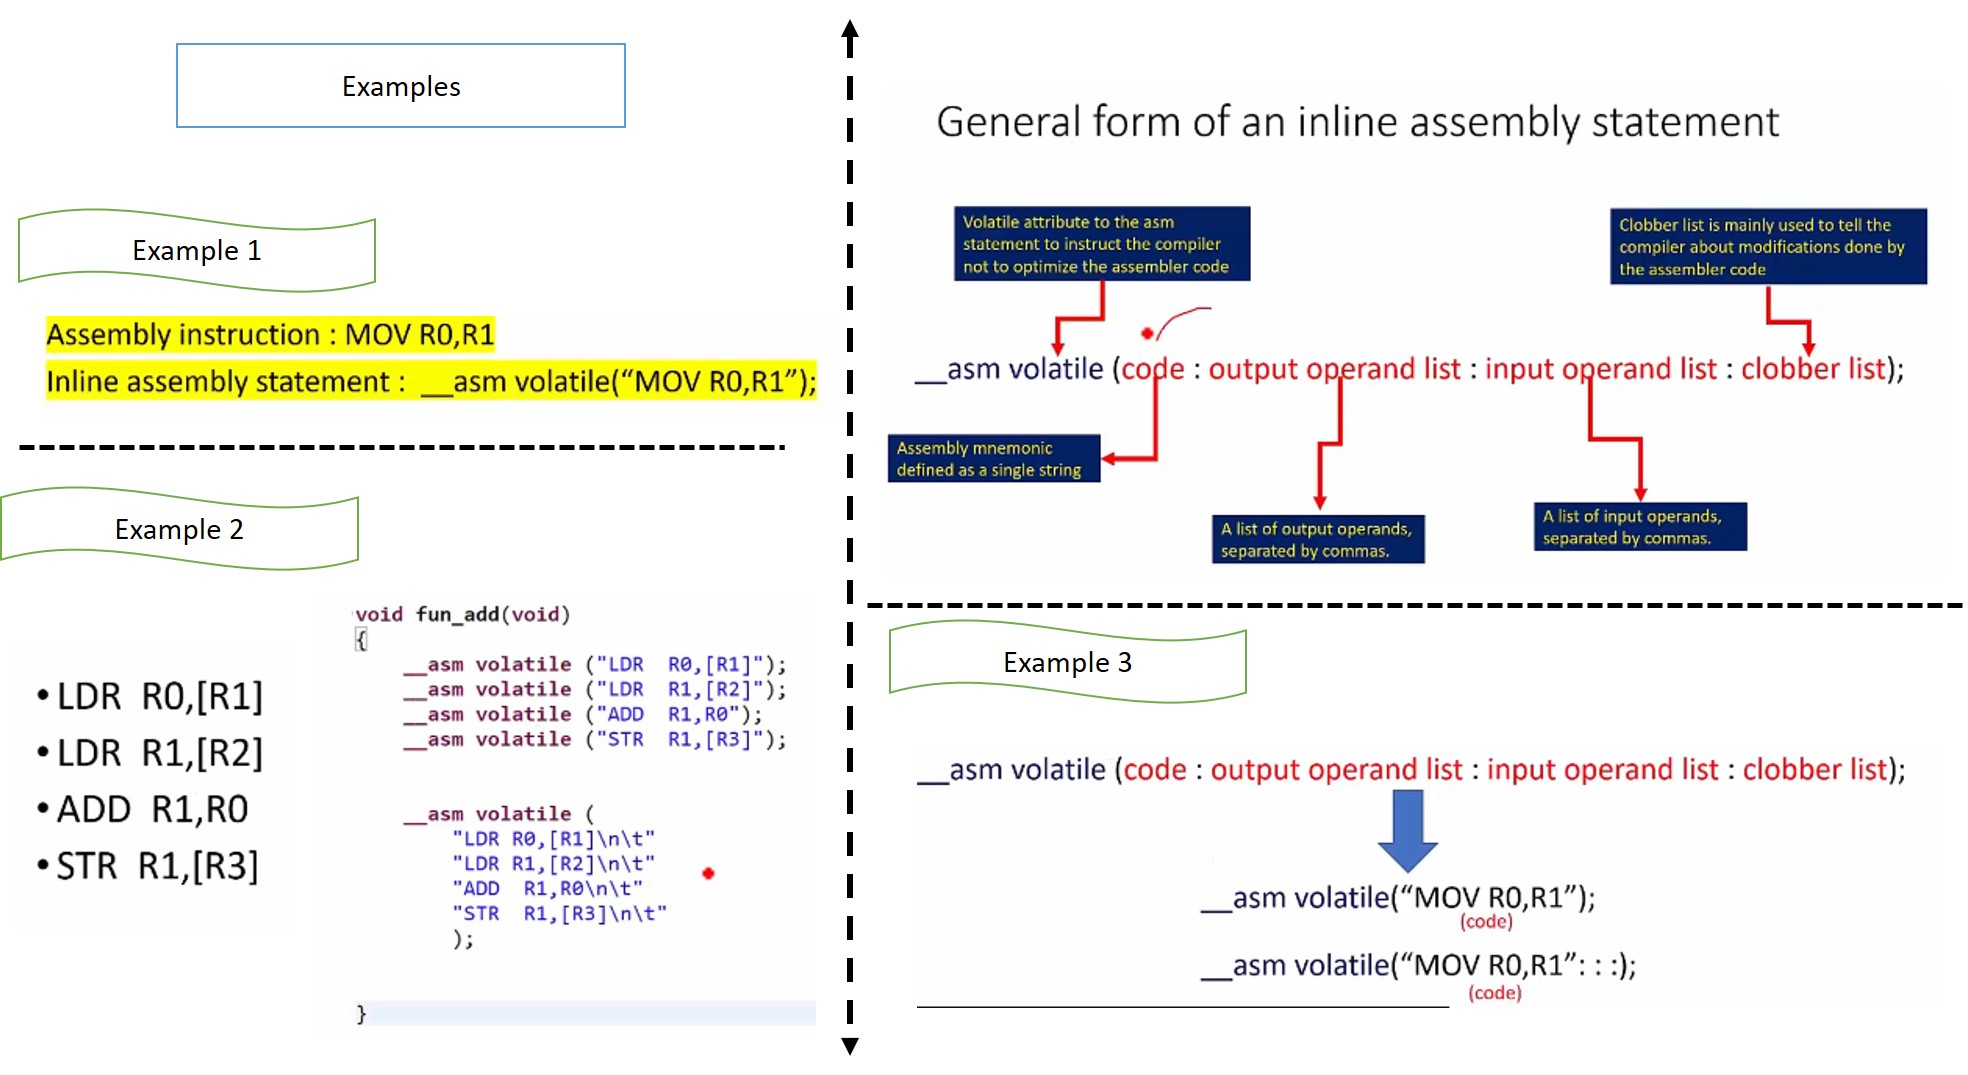
\includegraphics[scale=0.55]{Figures/ARM_Cortex/Inline_Assembly_example_syntax}
\caption{Inline Assembly: Examples and General Syntax}
\label{fig:ARM_Cortex:Inline_Assembly_example_syntax}
\end{figure}


\begin{itemize}
    \item We always begin with a leading double underscore

    \item In example 1: we embrace the code by " " and terminate it by a \verb|;|

    \item Example 2 shows 2 different syntax: the $\mathrm{2}^\mathrm{nd}$ one is more compact

        \begin{itemize}
            \item But notice no \verb|;| as in the $\mathrm{1}^\mathrm{st}$
        \end{itemize}

      \item In all the examples, there is only the code par: no operands and no clobber  
    
\end{itemize}

\subsection{Code Ex 1}

\underline{Given:} Load 2 values from memory, add them and store the result back into the memory using inline assembly language. \\

\todo{Code Demo} \underline{\textit{Code Demo}:} \textit{There is next some simple code demo illustrating the language, nothing important, maybe to do it later. This is done in video 29}. 


\subsection{Code Ex 2: C to ARM Reg}

\underline{Given:} Move the content of \verb|C| variable to ARM reg.\\

In this type of exercise, we will use input operand, and not just code section. The code is shown in \autoref{fig:ARM_Cortex:c_to_arm_reg}.


\begin{figure}[h]
\centering
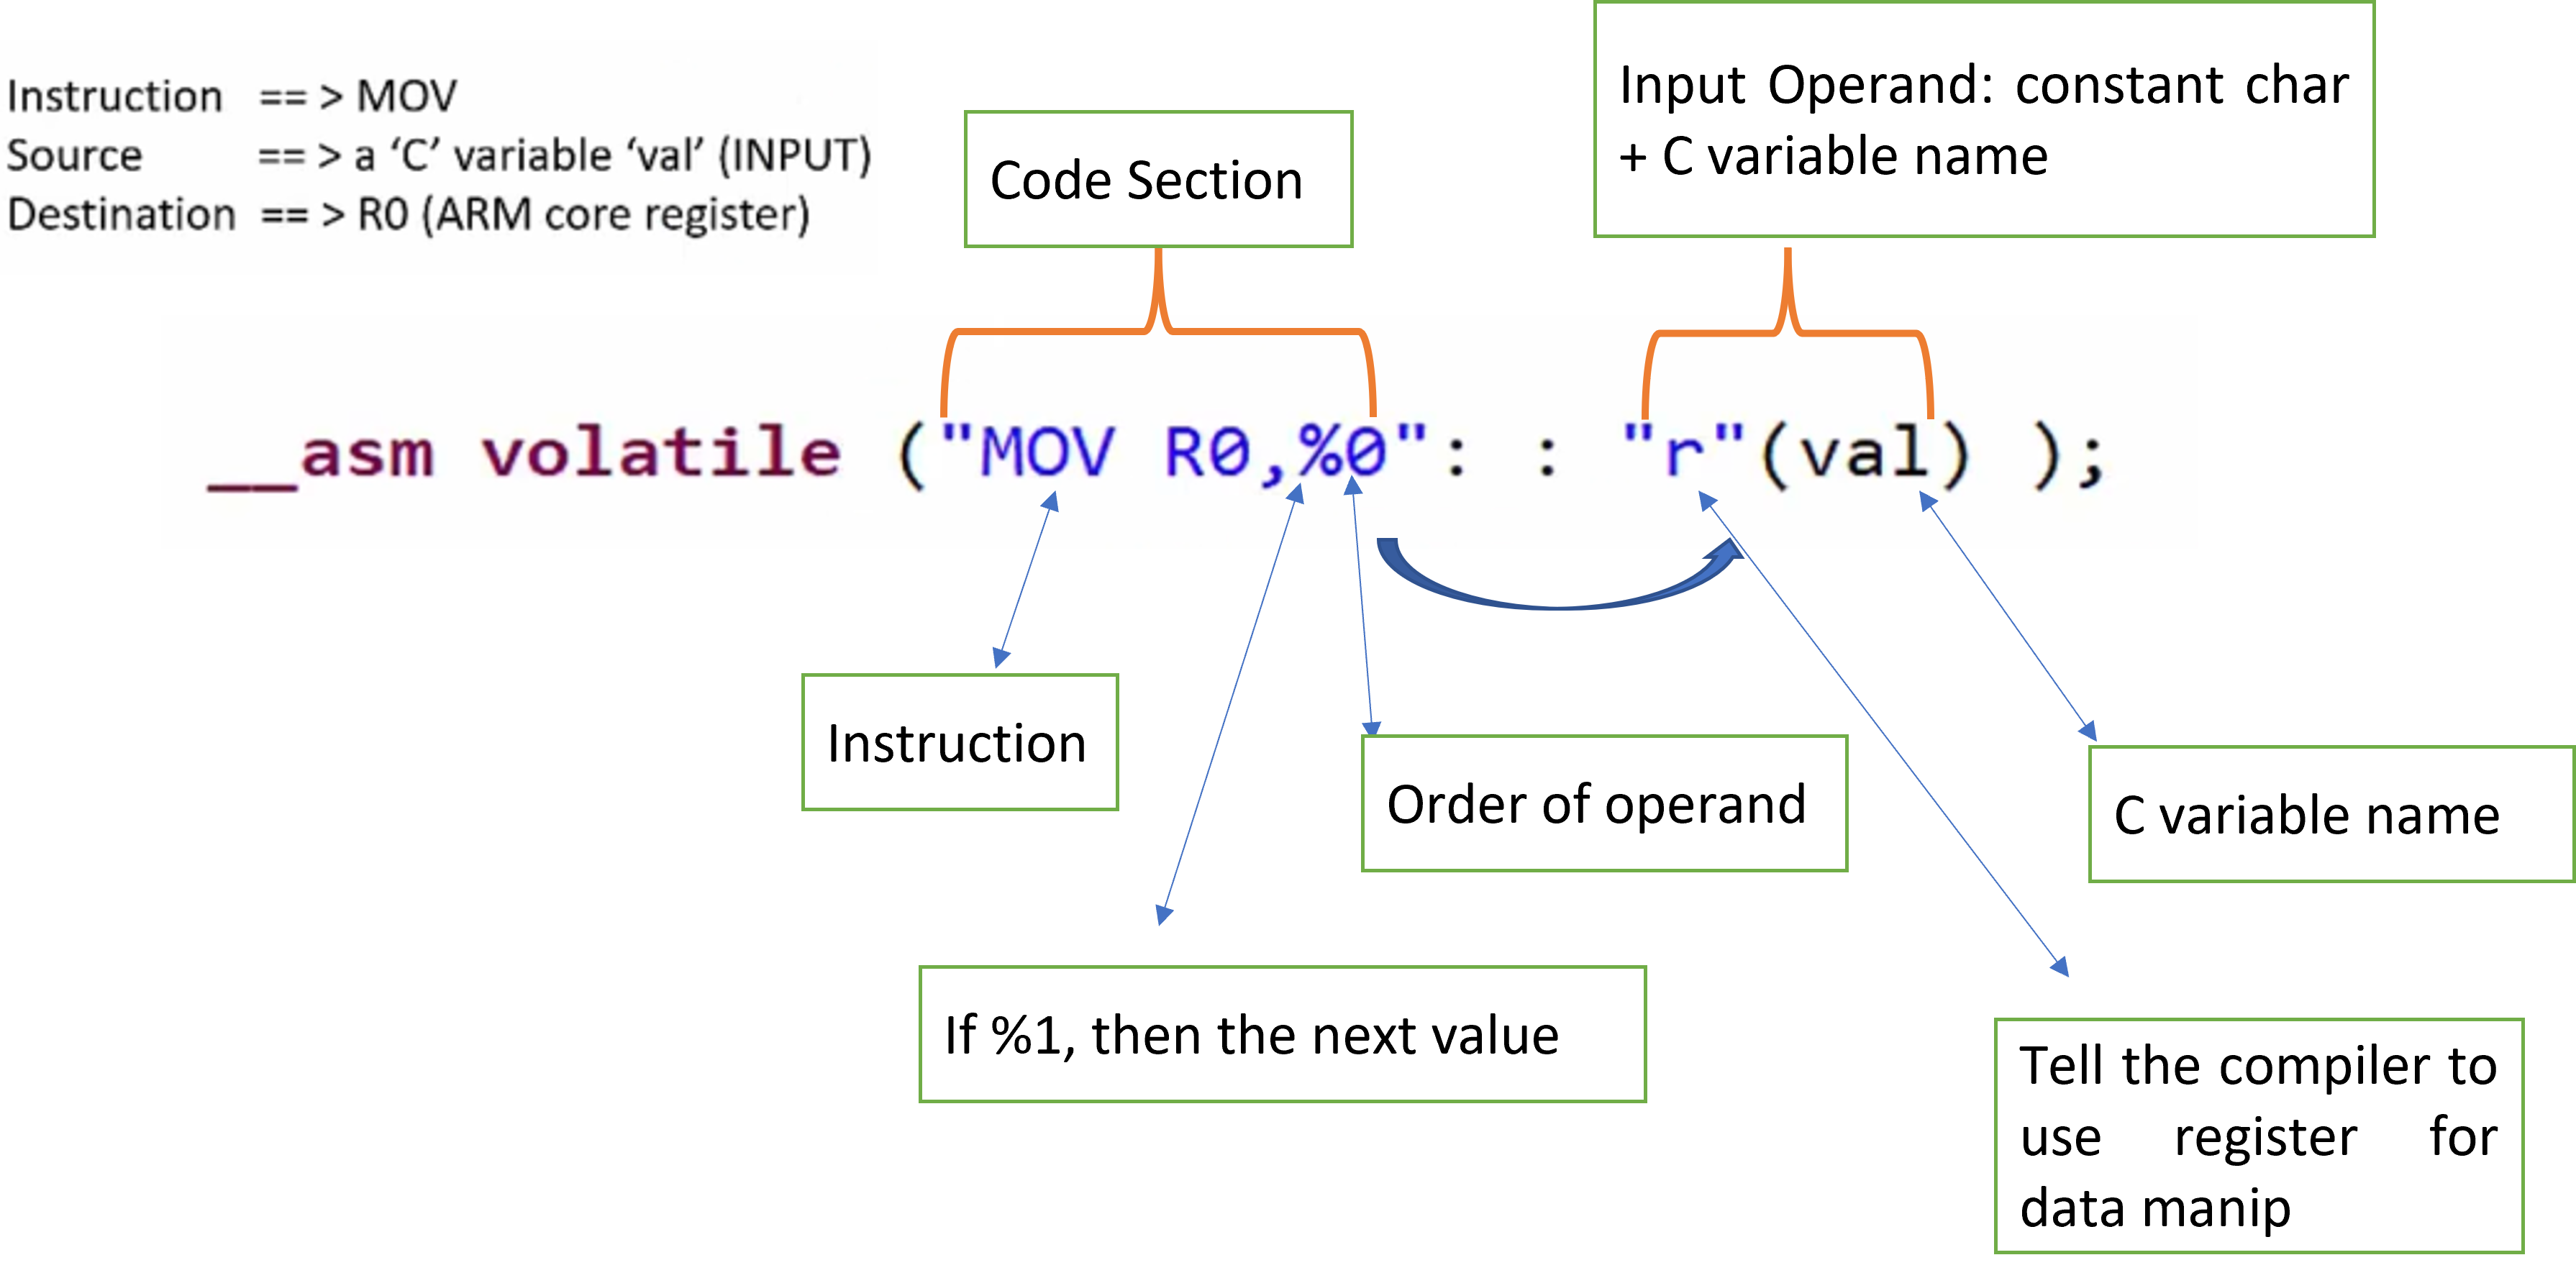
\includegraphics[scale=0.55]{Figures/ARM_Cortex/c_to_arm_reg}
\caption{C to ARM Register}
\label{fig:ARM_Cortex:c_to_arm_reg}
\end{figure}



\newpage
In order to see different constant character other then \verb|r|, contains all possibilities.


\begin{figure}[h]
\centering
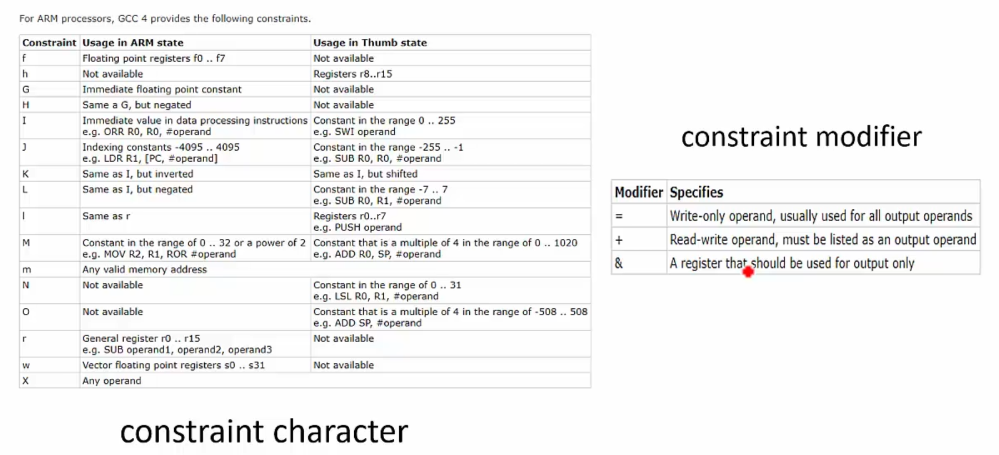
\includegraphics[scale=0.9]{Figures/ARM_Cortex/constraint_char_assembly}
\caption{Different constraint character}
\label{fig:ARM_Cortex:constraint_char_assembly}
\end{figure}

\subsection{ARM to C variable}

\underline{Given:} Move the content of \verb|CONTROL| reg to \verb|C| variable \verb|control-reg|.\\

In this exercise, we can see that \verb|C| variable is in the output operand, as shown in \autoref{fig:ARM_Cortex:arm_reg_to_c}

\begin{figure}[h]
\centering
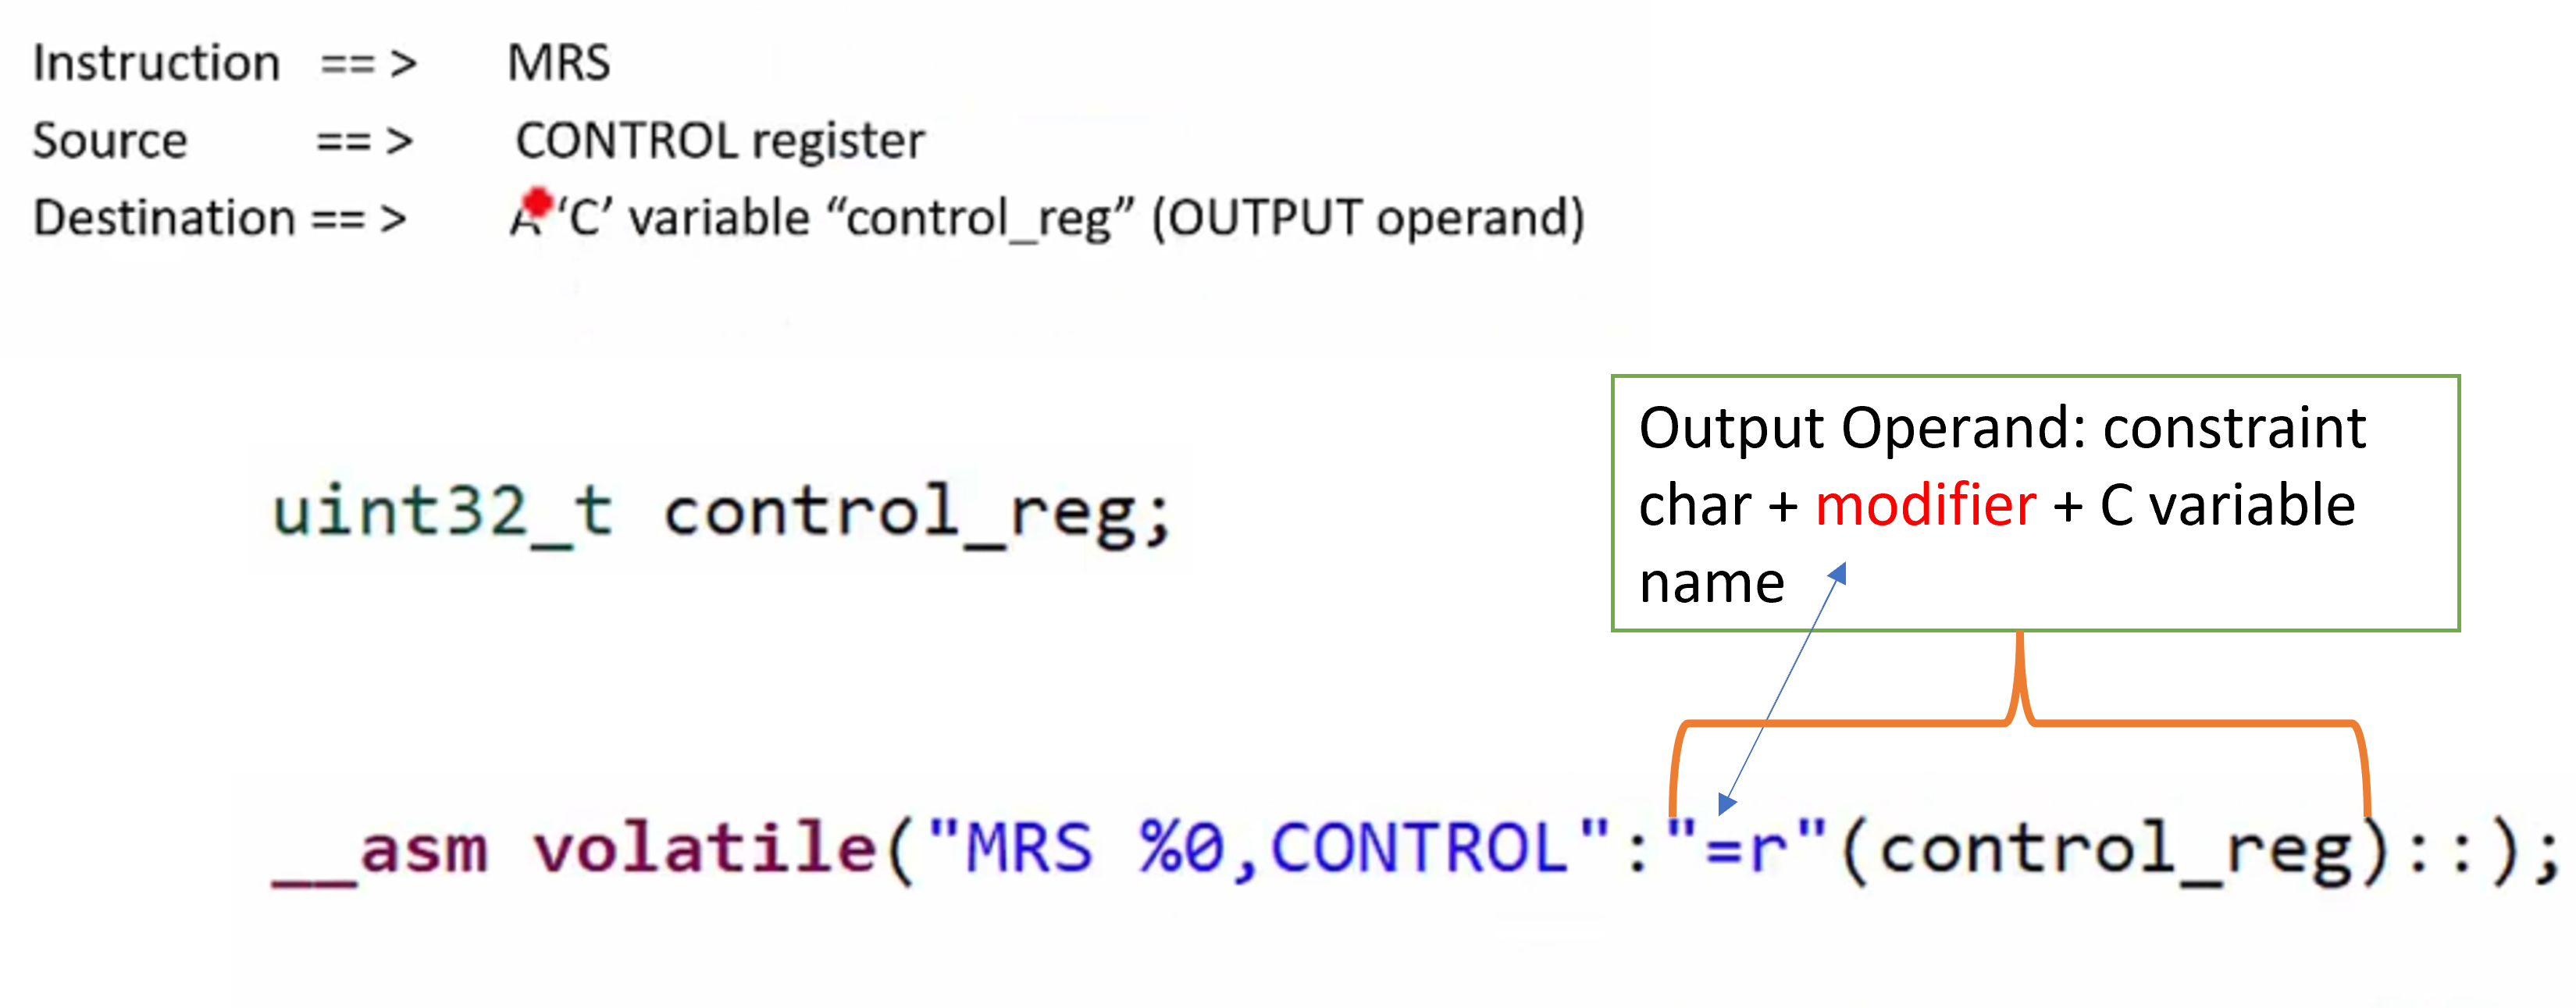
\includegraphics[scale=0.55]{Figures/ARM_Cortex/arm_reg_to_c}
\caption{C to ARM Register}
\label{fig:ARM_Cortex:arm_reg_to_c}
\end{figure}

\begin{itemize}
    \item We use the constraint modifier \verb|=| to indicate a write operation
\end{itemize}

\todo{Extra Ass Examples} \underline{\textit{Extra Ass Examples}:} \textit{There are some extra examples also, maybe see them later}.

\newpage

\section{Reset Sequence}

Now in this section, we discuss what happens when we press the reset button in our board: its mechanism, and what happen behind the scenes.\\

The reset handler function:

\begin{enumerate}
    \item doing some initialization


    \item Call the \verb|main| function
\end{enumerate}


\autoref{fig:ARM_Cortex:reset_handler_job} shows this concept.

\begin{figure}[h]
\centering
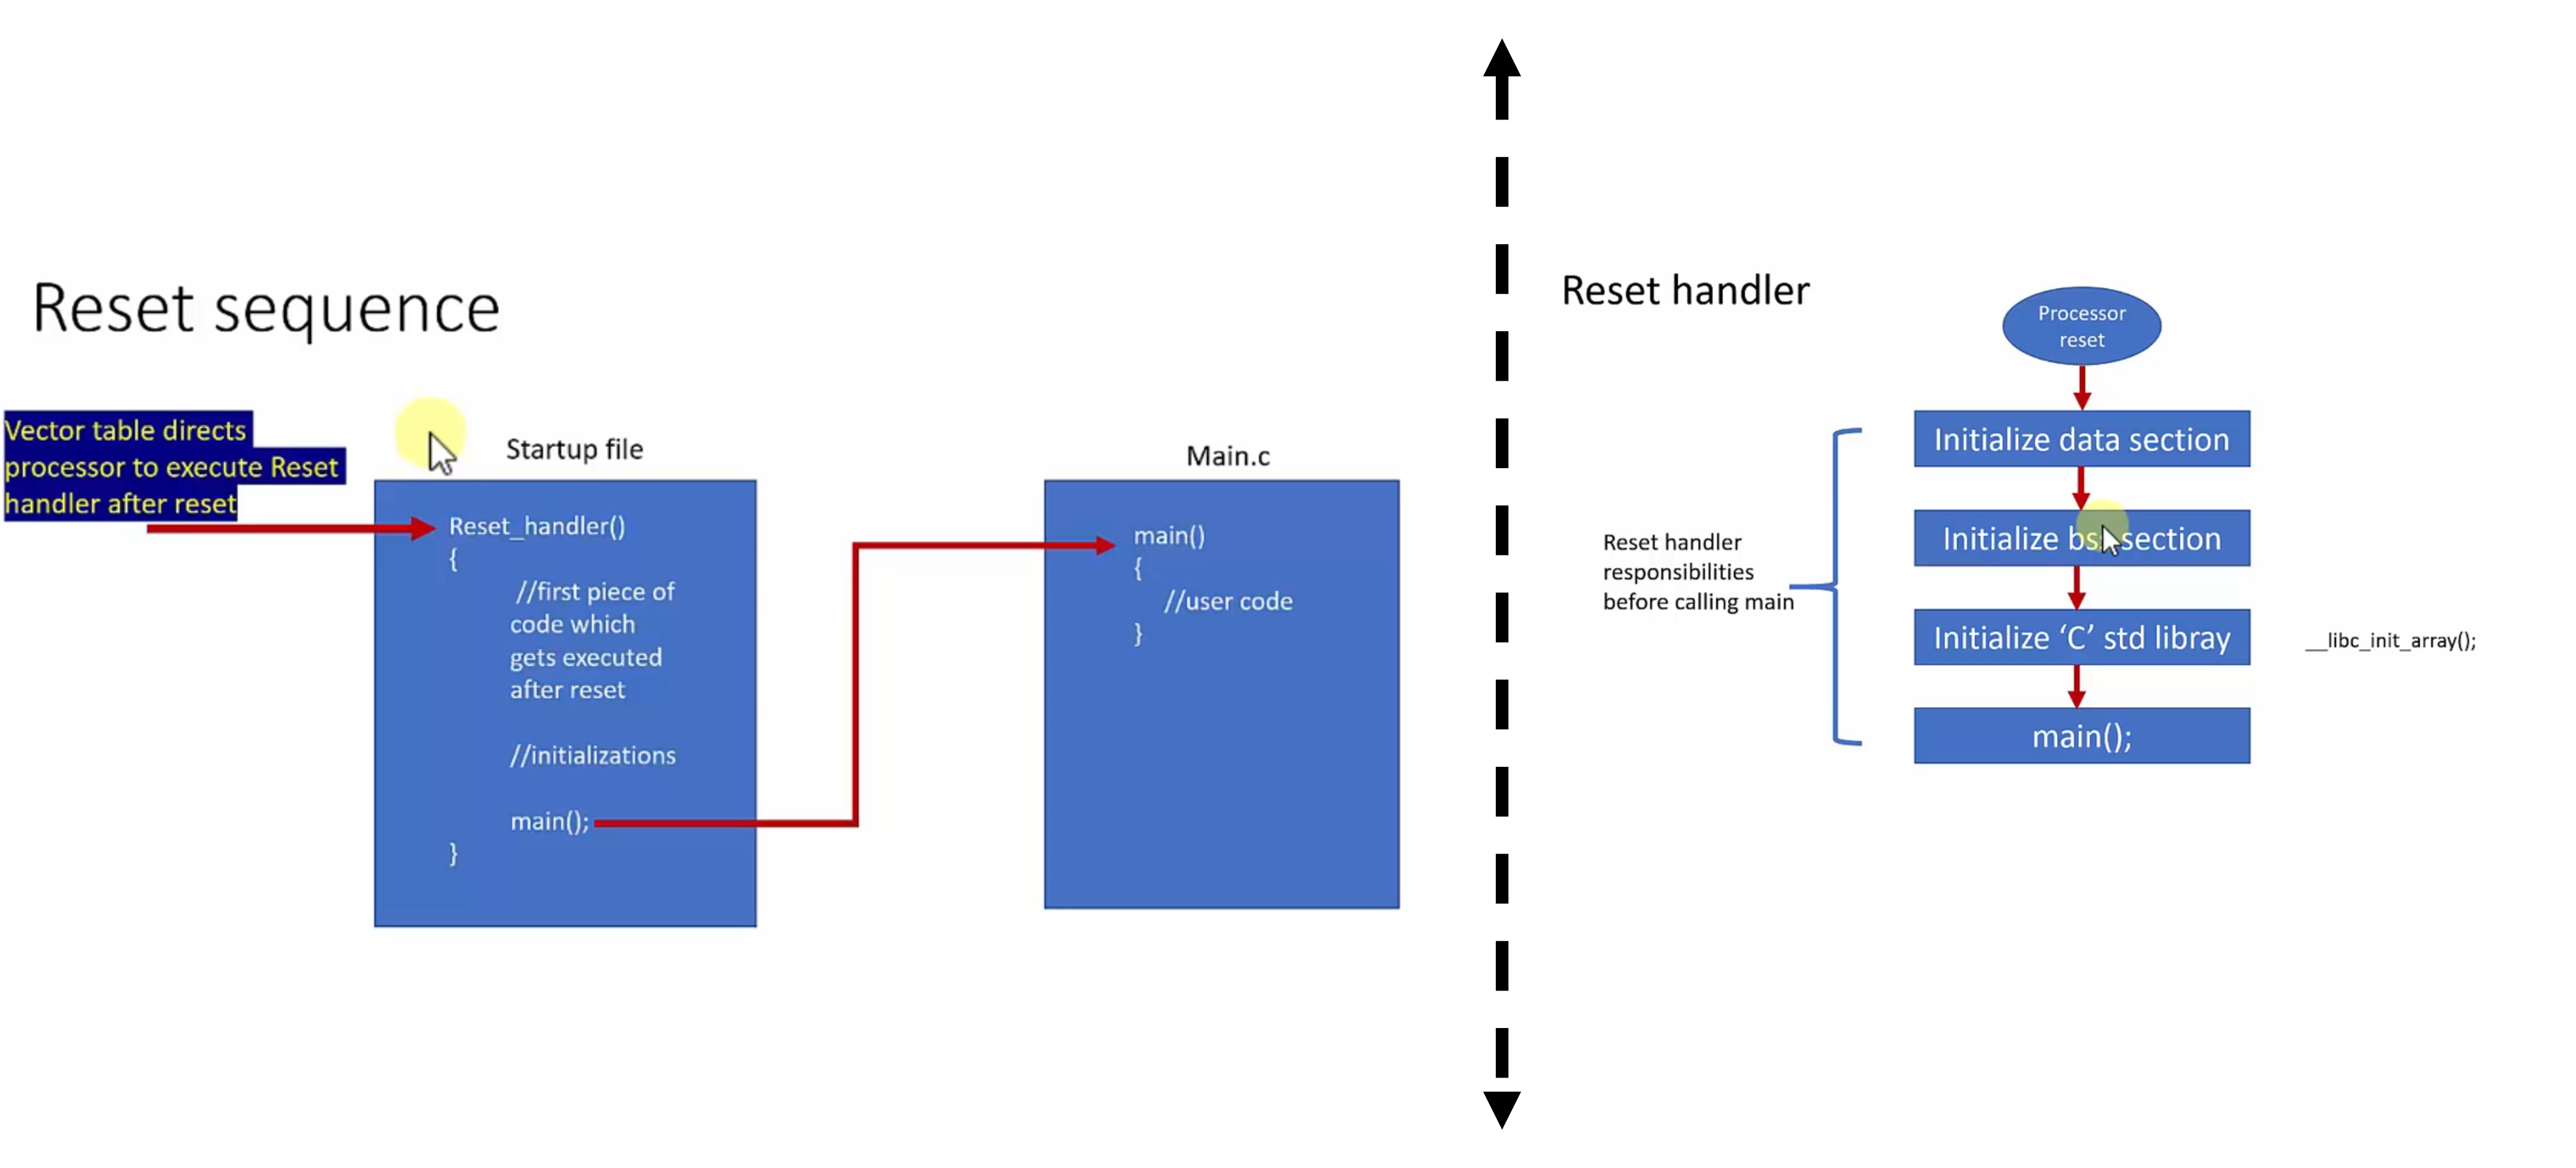
\includegraphics[scale=0.55]{Figures/ARM_Cortex/reset_handler_job}
\caption{Reset Handler Task}
\label{fig:ARM_Cortex:reset_handler_job}
\end{figure}


Now as regarding the steps, \autoref{fig:ARM_Cortex:reset_handler_steps_with_reg} illustrate this steps from register side:

\begin{figure}[h]
\centering
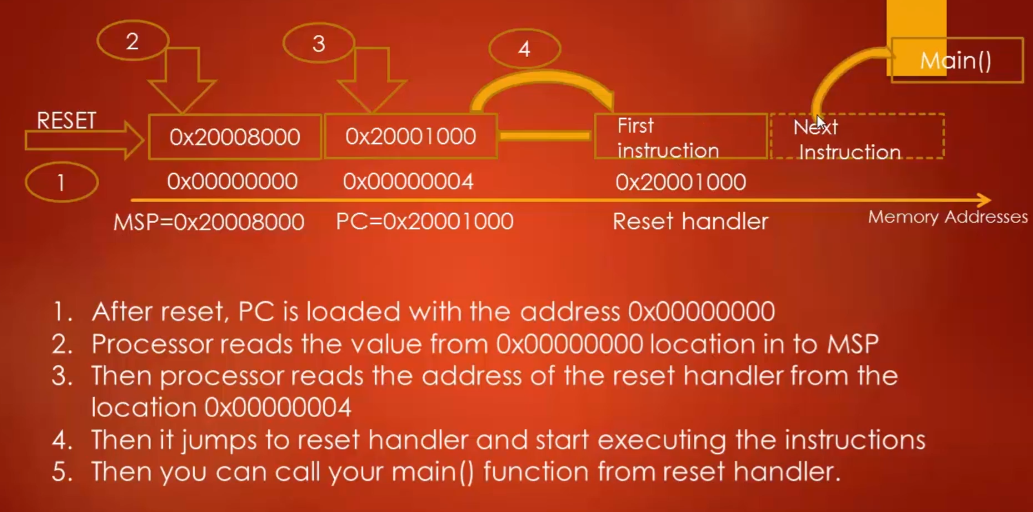
\includegraphics[scale=0.55]{Figures/ARM_Cortex/reset_handler_steps_with_reg}
\caption{Reset Handler steps with registers}
\label{fig:ARM_Cortex:reset_handler_steps_with_reg}
\end{figure}

\begin{itemize}

    \item \underline{Registers:} \verb|MSP|: memory stack pointer , \verb|PC|: program counter
    
    \item Notice that \verb|PC| stores the address of \verb|Reset| function which is 0x20001000 at location 0x0000 0004.
\end{itemize}


\newpage

\section{Demo for Access Level}

Now in this section, we see how to change access level.

\underline{Review:}

\begin{itemize}
    \item We know from \autoref{Sec:Operations_Modes} that the code starts in thread mode, with PAL access.


    \item In the demo code of \ref{Sub:Operation_Mode_Demo}, we switch the code from thread mode to handler mode using an interrupt
\end{itemize}


Now the big idea about privilege and unprivileged mode:

\begin{itemize}
    \item Suppose we have some real time OS and some user task

    \item The user task shouldn't modify the kernel system (like switching off or ON a ISR)


    \item That's why sometimes we switch from thread mode PAL to thread model NPAL

    \item Because in NPAL we can't access the resources of the kernel and modify it
    
\end{itemize}

T bit in \verb|ESPR|: T bit should always set to 1.\\

\todo{T bit} \underline{\textit{T bit}:} \textit{To watch the video later about the T bit, thumb state and so on, and why ARM is in thumb state always. This is video 33 and 34 from section 8}. 

\newpage
\section{Memory Map}

In this section, we discuss memory map of the processor and processor communicates with different peripheral of the MCU. \autoref{fig:ARM_Cortex:memory_map_com_process_periph} shows block diagram about communication concepts: (a) using the bus interface), and the memory map part (b)

\begin{figure}[h]
\centering
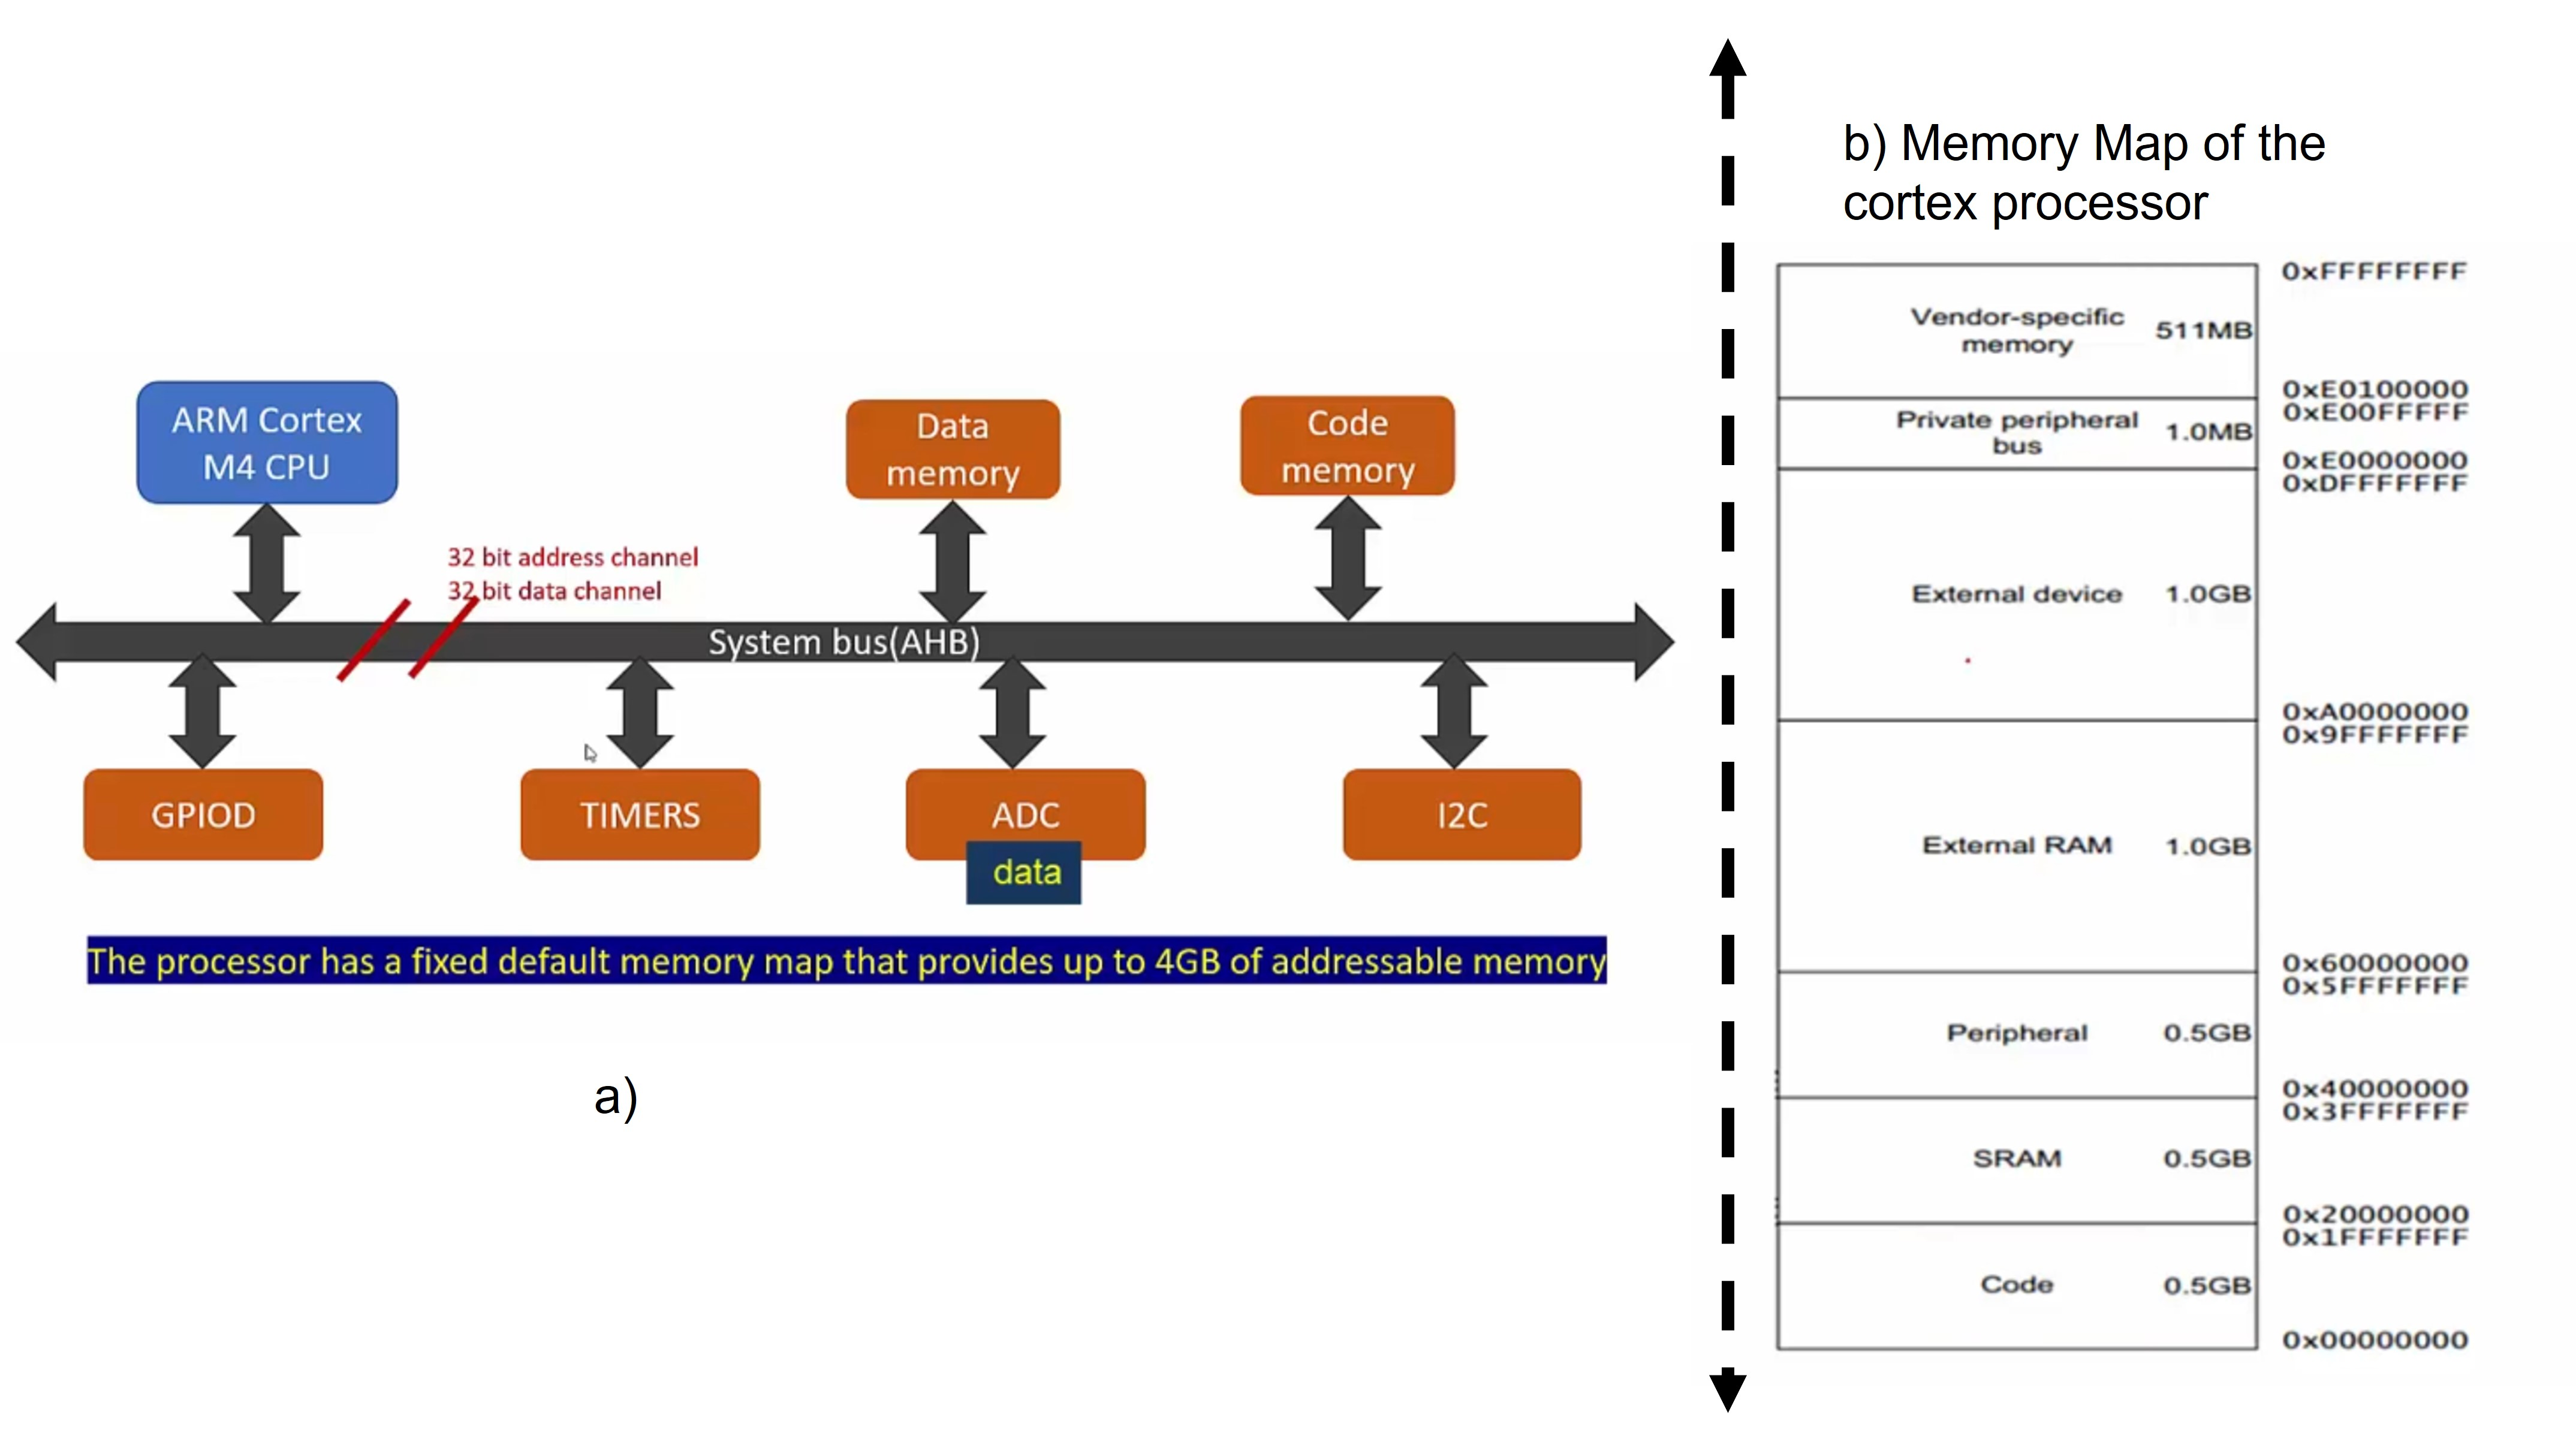
\includegraphics[scale=0.55]{Figures/ARM_Cortex/memory_map_com_process_periph}
\caption{Communication between Processor and different peripheral}
\label{fig:ARM_Cortex:memory_map_com_process_periph}
\end{figure}

Suppose that the ADC have some data in it, and we want to use this data in our software, so we need to store these data in the \textit{data memory}. The steps are:

\begin{enumerate}
    \item The processor generate addresses, and compare them to the address in which the data is hold in the ADC register (call it \verb|RegADC|)

    \begin{itemize}
        \item Here comes the role of the memory map. For example, when the processor wants to communicate with the ADC, the generated address should be in the peripheral range (0x4000 0000 $\rightarrow$ 0x5FFF FFFF)
    \end{itemize}

    \item Once the address of \verb|RegADC| is found, \verb|RegADC| will be unlocked and its content (the data we need)  will be sent using the data bus to the processor, and stored in some register of the processor 

    \item The move it to the Data peripheral part
\end{enumerate}
    
These steps can be summarized using 2 instructions:

\begin{enumerate}
    \item \verb|load| instruction from the ADC to the processor

    \item \verb|store| instruction to store the data in the data memory
\end{enumerate}


One thing to be noted also: the peripheral space map range is used in the design when specifying the needed addresses of the peripheral of the MCU (such as timers,ADC,$\cdots$).

\subsection{Bus Interface}

From previous explanation, we can see that the communication is done using buses. IN ARM architecture, there are 2 bus:

\begin{enumerate}
    \item AHB bus:

    \begin{itemize}
        \item High speed communication with peripheral that demands high speed operation

        \item 
    \end{itemize}


    \item APB bus:

    \begin{itemize}
        \item Low speed communication

        \item For PPB (private peripheral bus region) such as NVIC, system timer,$\cdots$
    \end{itemize}
\end{enumerate}


\underline{Design Concept:} we have 2 bus (AHB and APB) because by this way, MCU vendors can put the peripheral which don't require high speed on low performance bus (the APB in our case) and reduce power consumption.


\subsection{Bit Banding Feature}

Now we explore a feature called \textit{bit banding}

\begin{itemize}
    \item Definition: capability to address a single bit of a memory address.

    \item Not all memory map are bit banded. As shown in \autoref{fig:ARM_Cortex:bit_banding_memory_map}, only SRAM and the peripheral sections are bit banded. 


\begin{figure}[h]
\centering
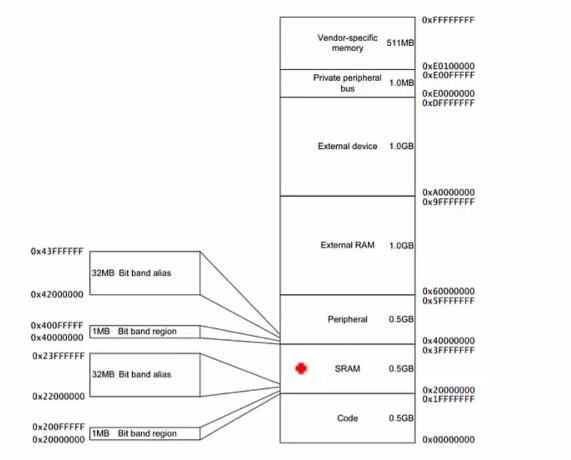
\includegraphics[scale=0.7]{Figures/ARM_Cortex/bit_banding_memory_map}
\caption{Bit banding: allowed section of the memory map}
\label{fig:ARM_Cortex:bit_banding_memory_map}
\end{figure}

\newpage
\item How to address the bits: via the equivalent alias address as shown in \autoref{fig:ARM_Cortex:bit_banding_mechanism}.

\begin{figure}[h]
\centering
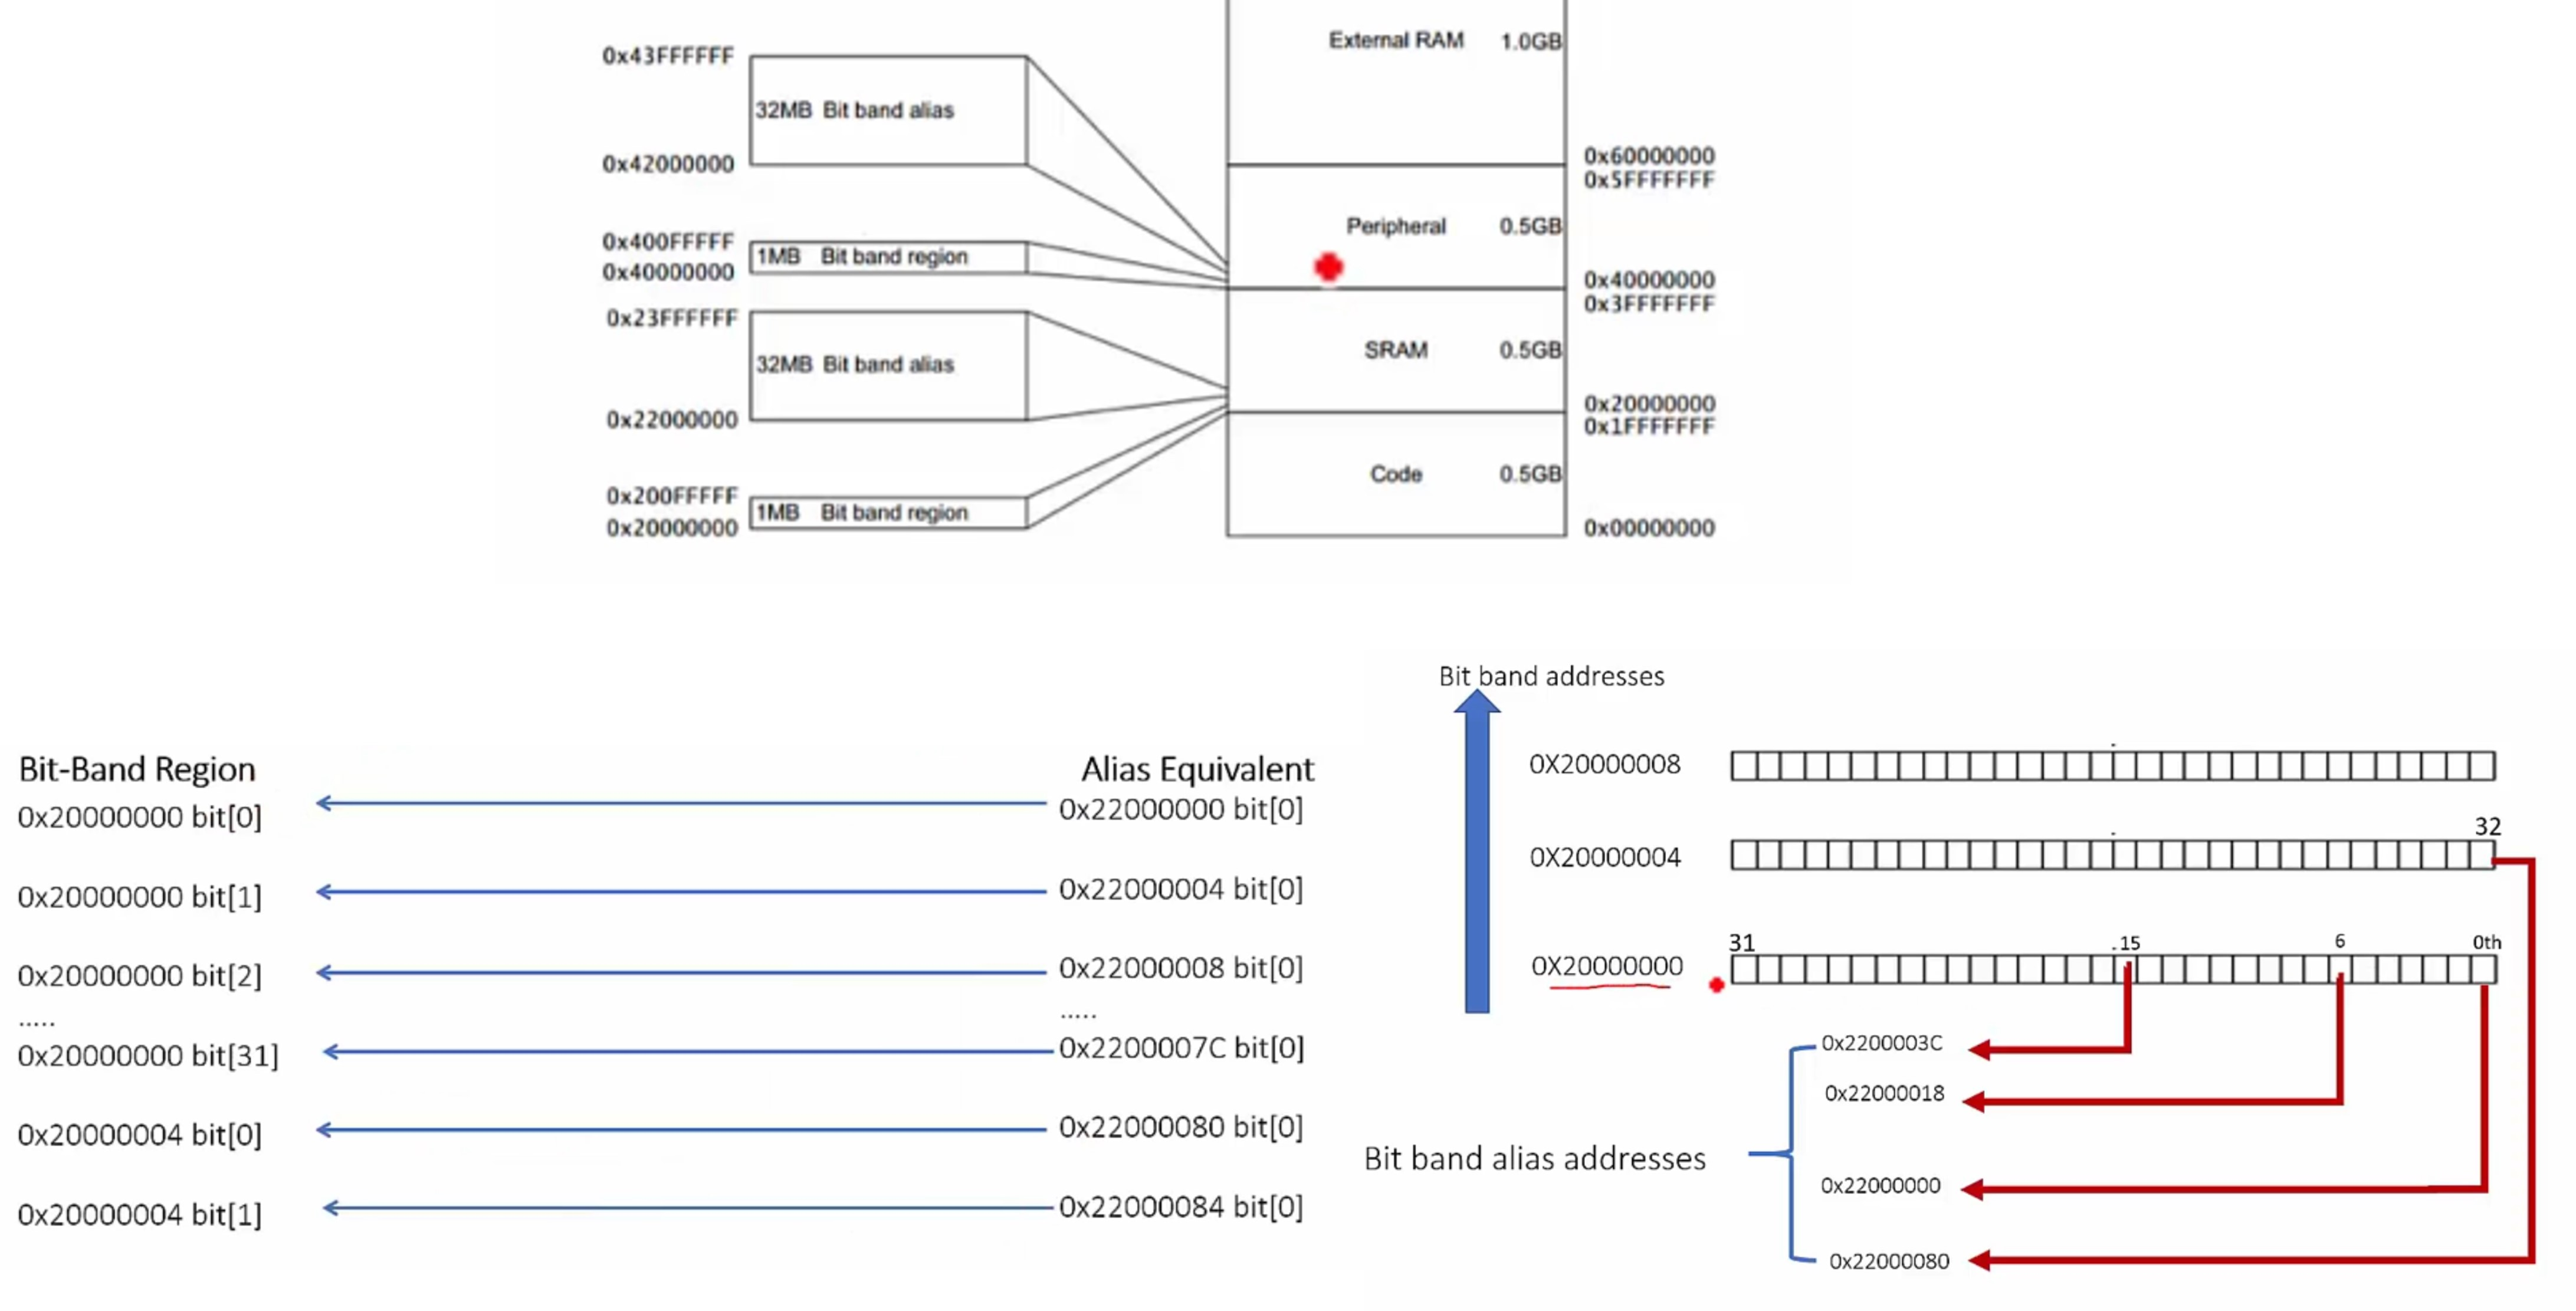
\includegraphics[scale=0.5]{Figures/ARM_Cortex/bit_banding_mechanism}
\caption{Bit banding mechanism}
\label{fig:ARM_Cortex:bit_banding_mechanism}
\end{figure}

For each bit, correspond an alias address.
    
\end{itemize}


\todo{Bit banding code} \underline{\textit{Bit banding code}:} \textit{to redo the coding exercise later. See video 38 section 9}. 

\newpage
\section{Stack}

\underline{Main Concepts:}

\begin{itemize}

\item Stack is a memory used when executing functions,or interrupts/exception, and also to store variables

\item Stack operation mode: they are general 4 operation mode as seen in \autoref{fig:ARM_Cortex:stack_operation_modes}


\begin{figure}[h]
\centering
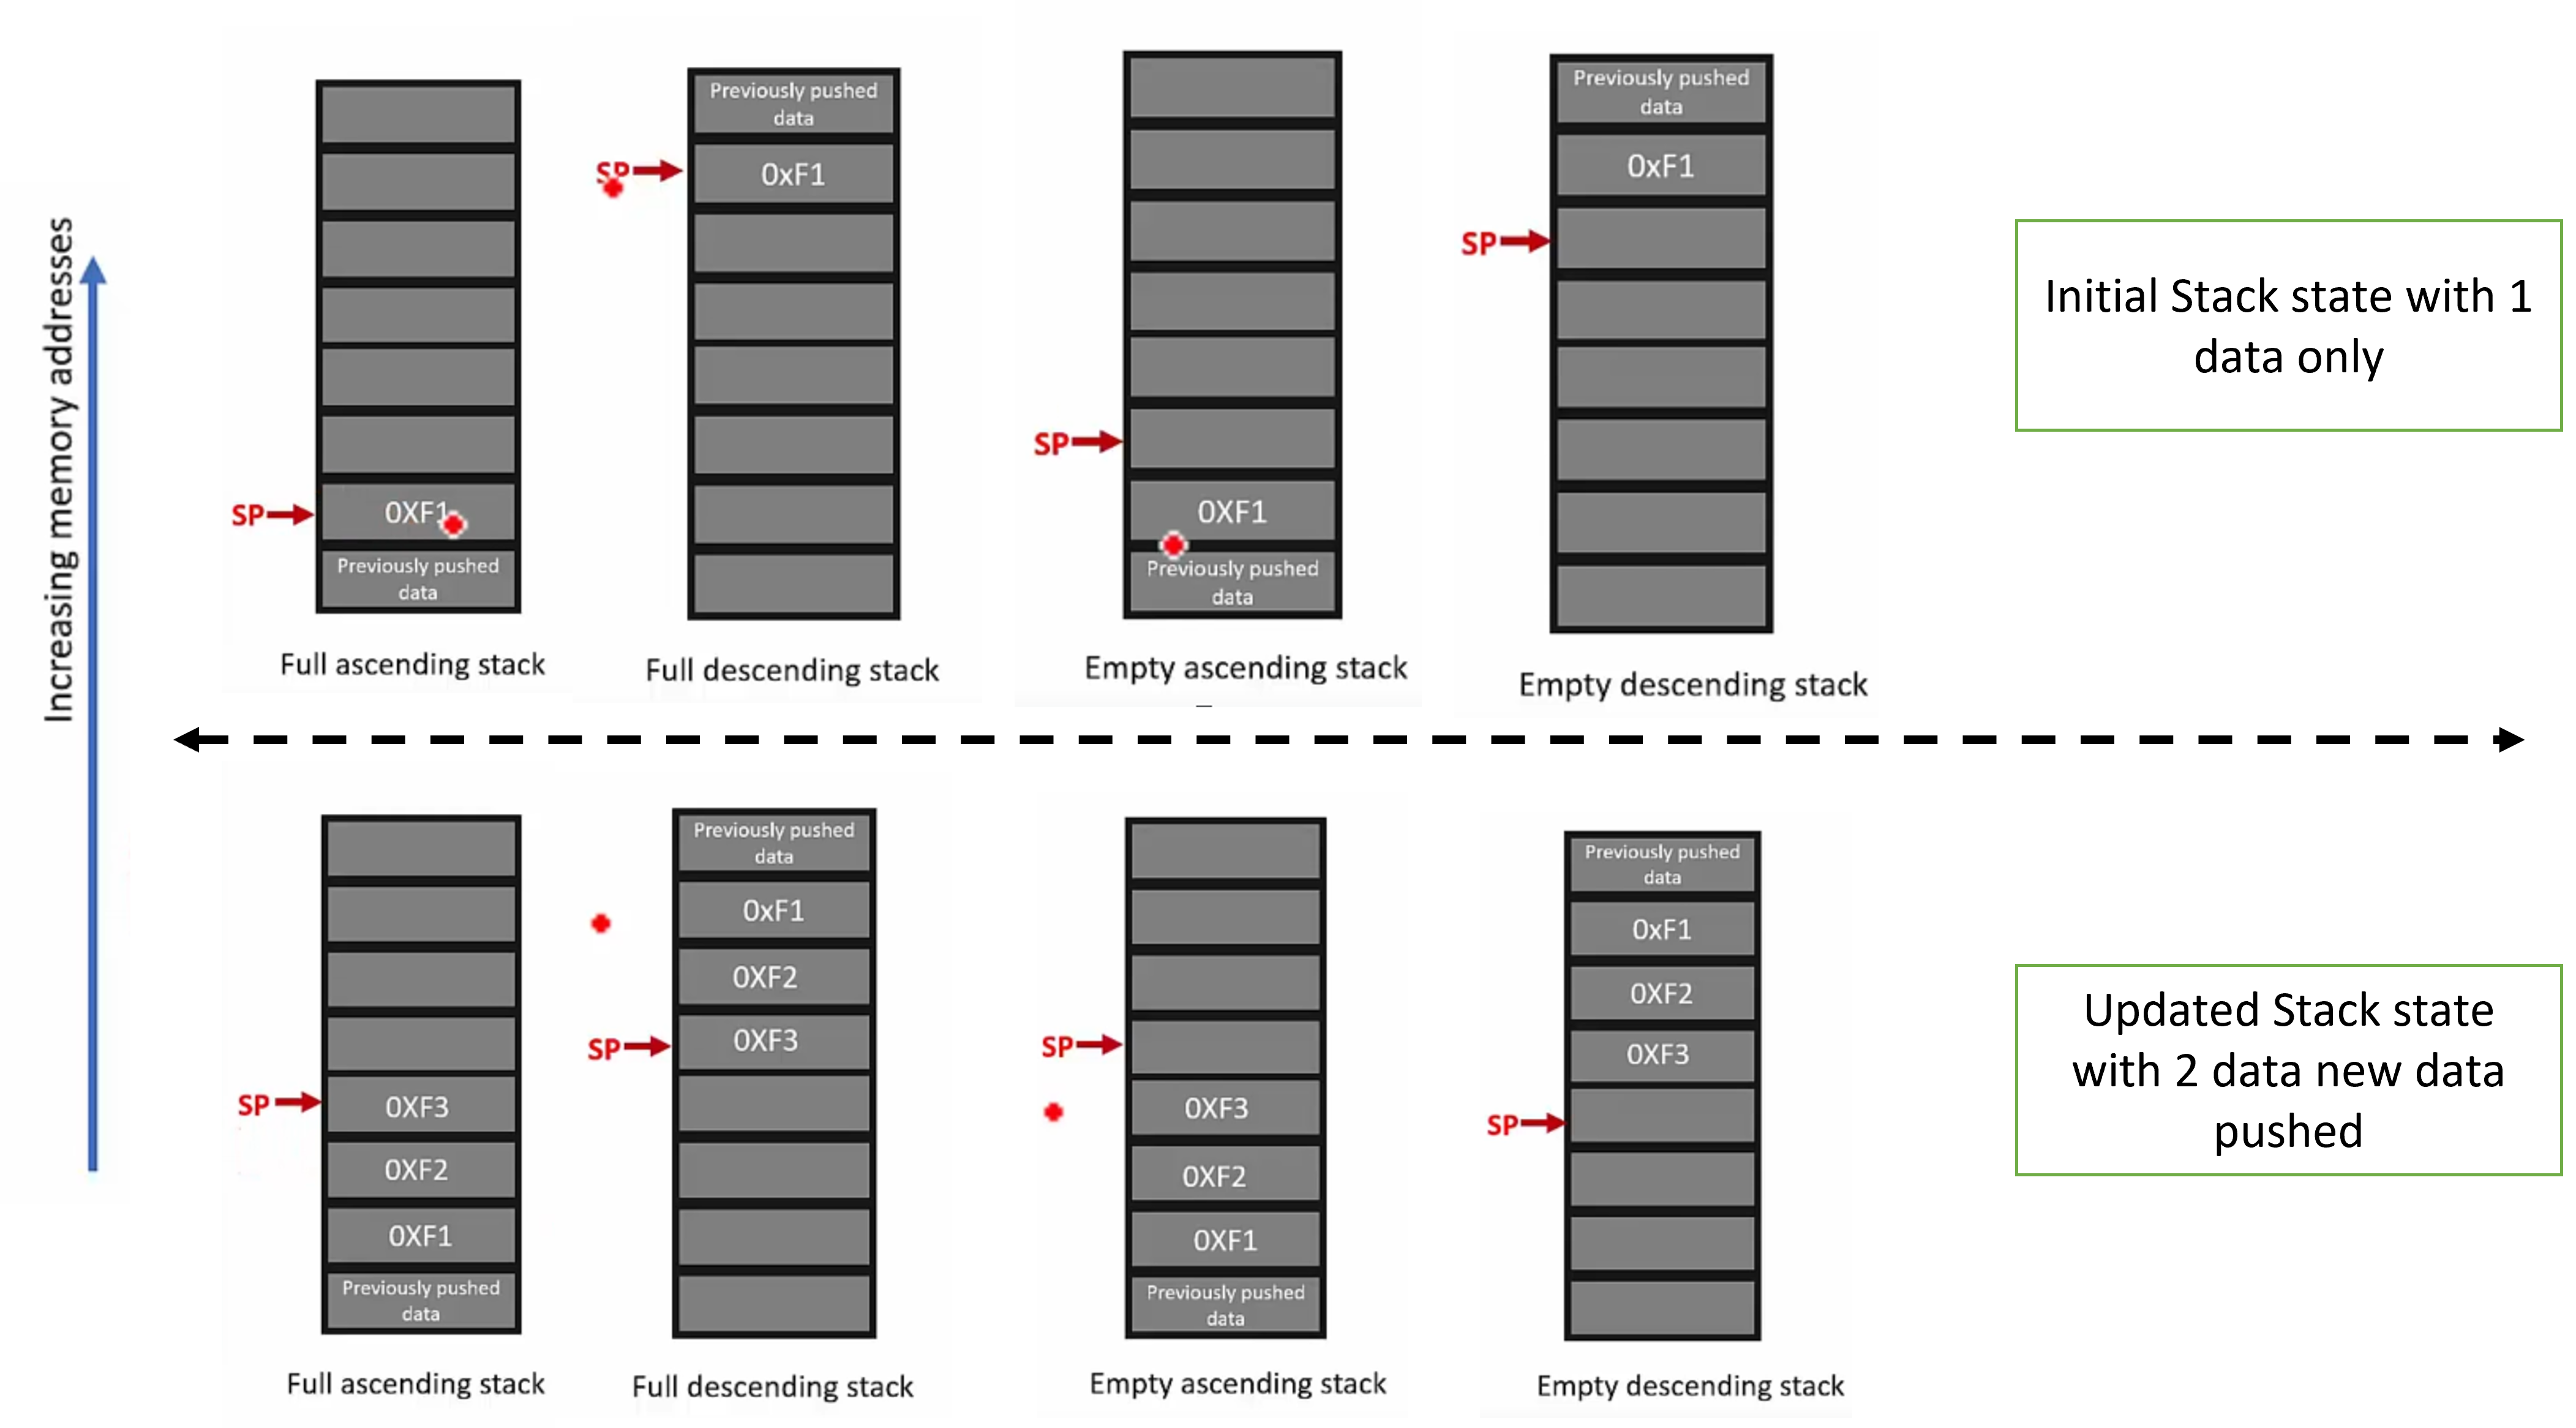
\includegraphics[scale=0.5]{Figures/ARM_Cortex/stack_operation_modes}
\caption{Stack Operation Mode}
\label{fig:ARM_Cortex:stack_operation_modes}
\end{figure}

\begin{itemize}
    \item Ascending mode: \verb|SP| is increasing

    \item Empty mode: \verb|SP| points toward empty memory address (ascending and descending mode)
\end{itemize}


In arm cortex, we use full descending


\newpage

\item Stack placement: we can place the stack in many ways as shown in \autoref{fig:ARM_Cortex:stack_placement}. Usually we use the $\mathrm{2}^\mathrm{nd}$ one.


\begin{figure}[h]
\centering
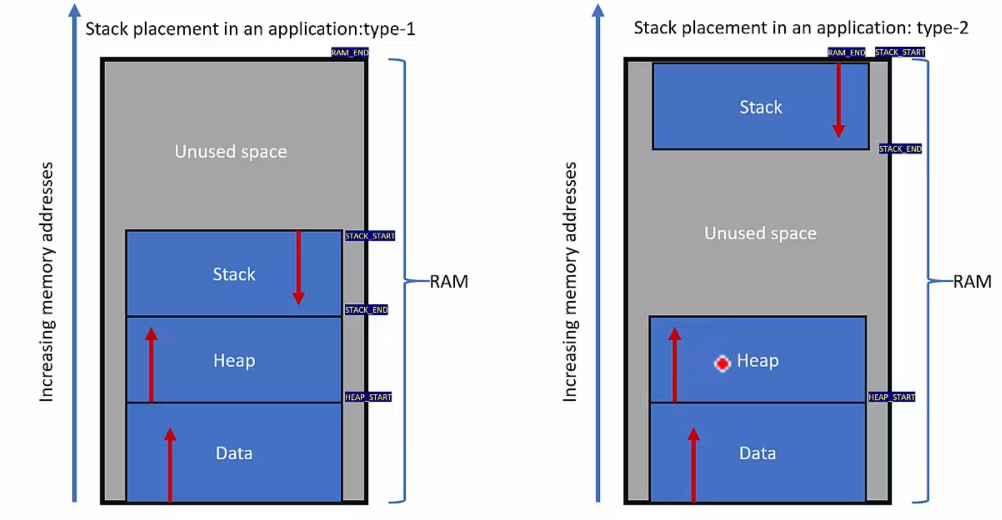
\includegraphics[scale=0.5]{Figures/ARM_Cortex/stack_placement}
\caption{Stack Operation Mode}
\label{fig:ARM_Cortex:stack_placement}
\end{figure}


\item Bank stack pointer: if we go to the user guide of the cortex M4 processor, we see that at \verb|R13| we have a bank of pointers as shown in \autoref{fig:ARM_Cortex:bank_stack}.

\begin{figure}[h]
\centering
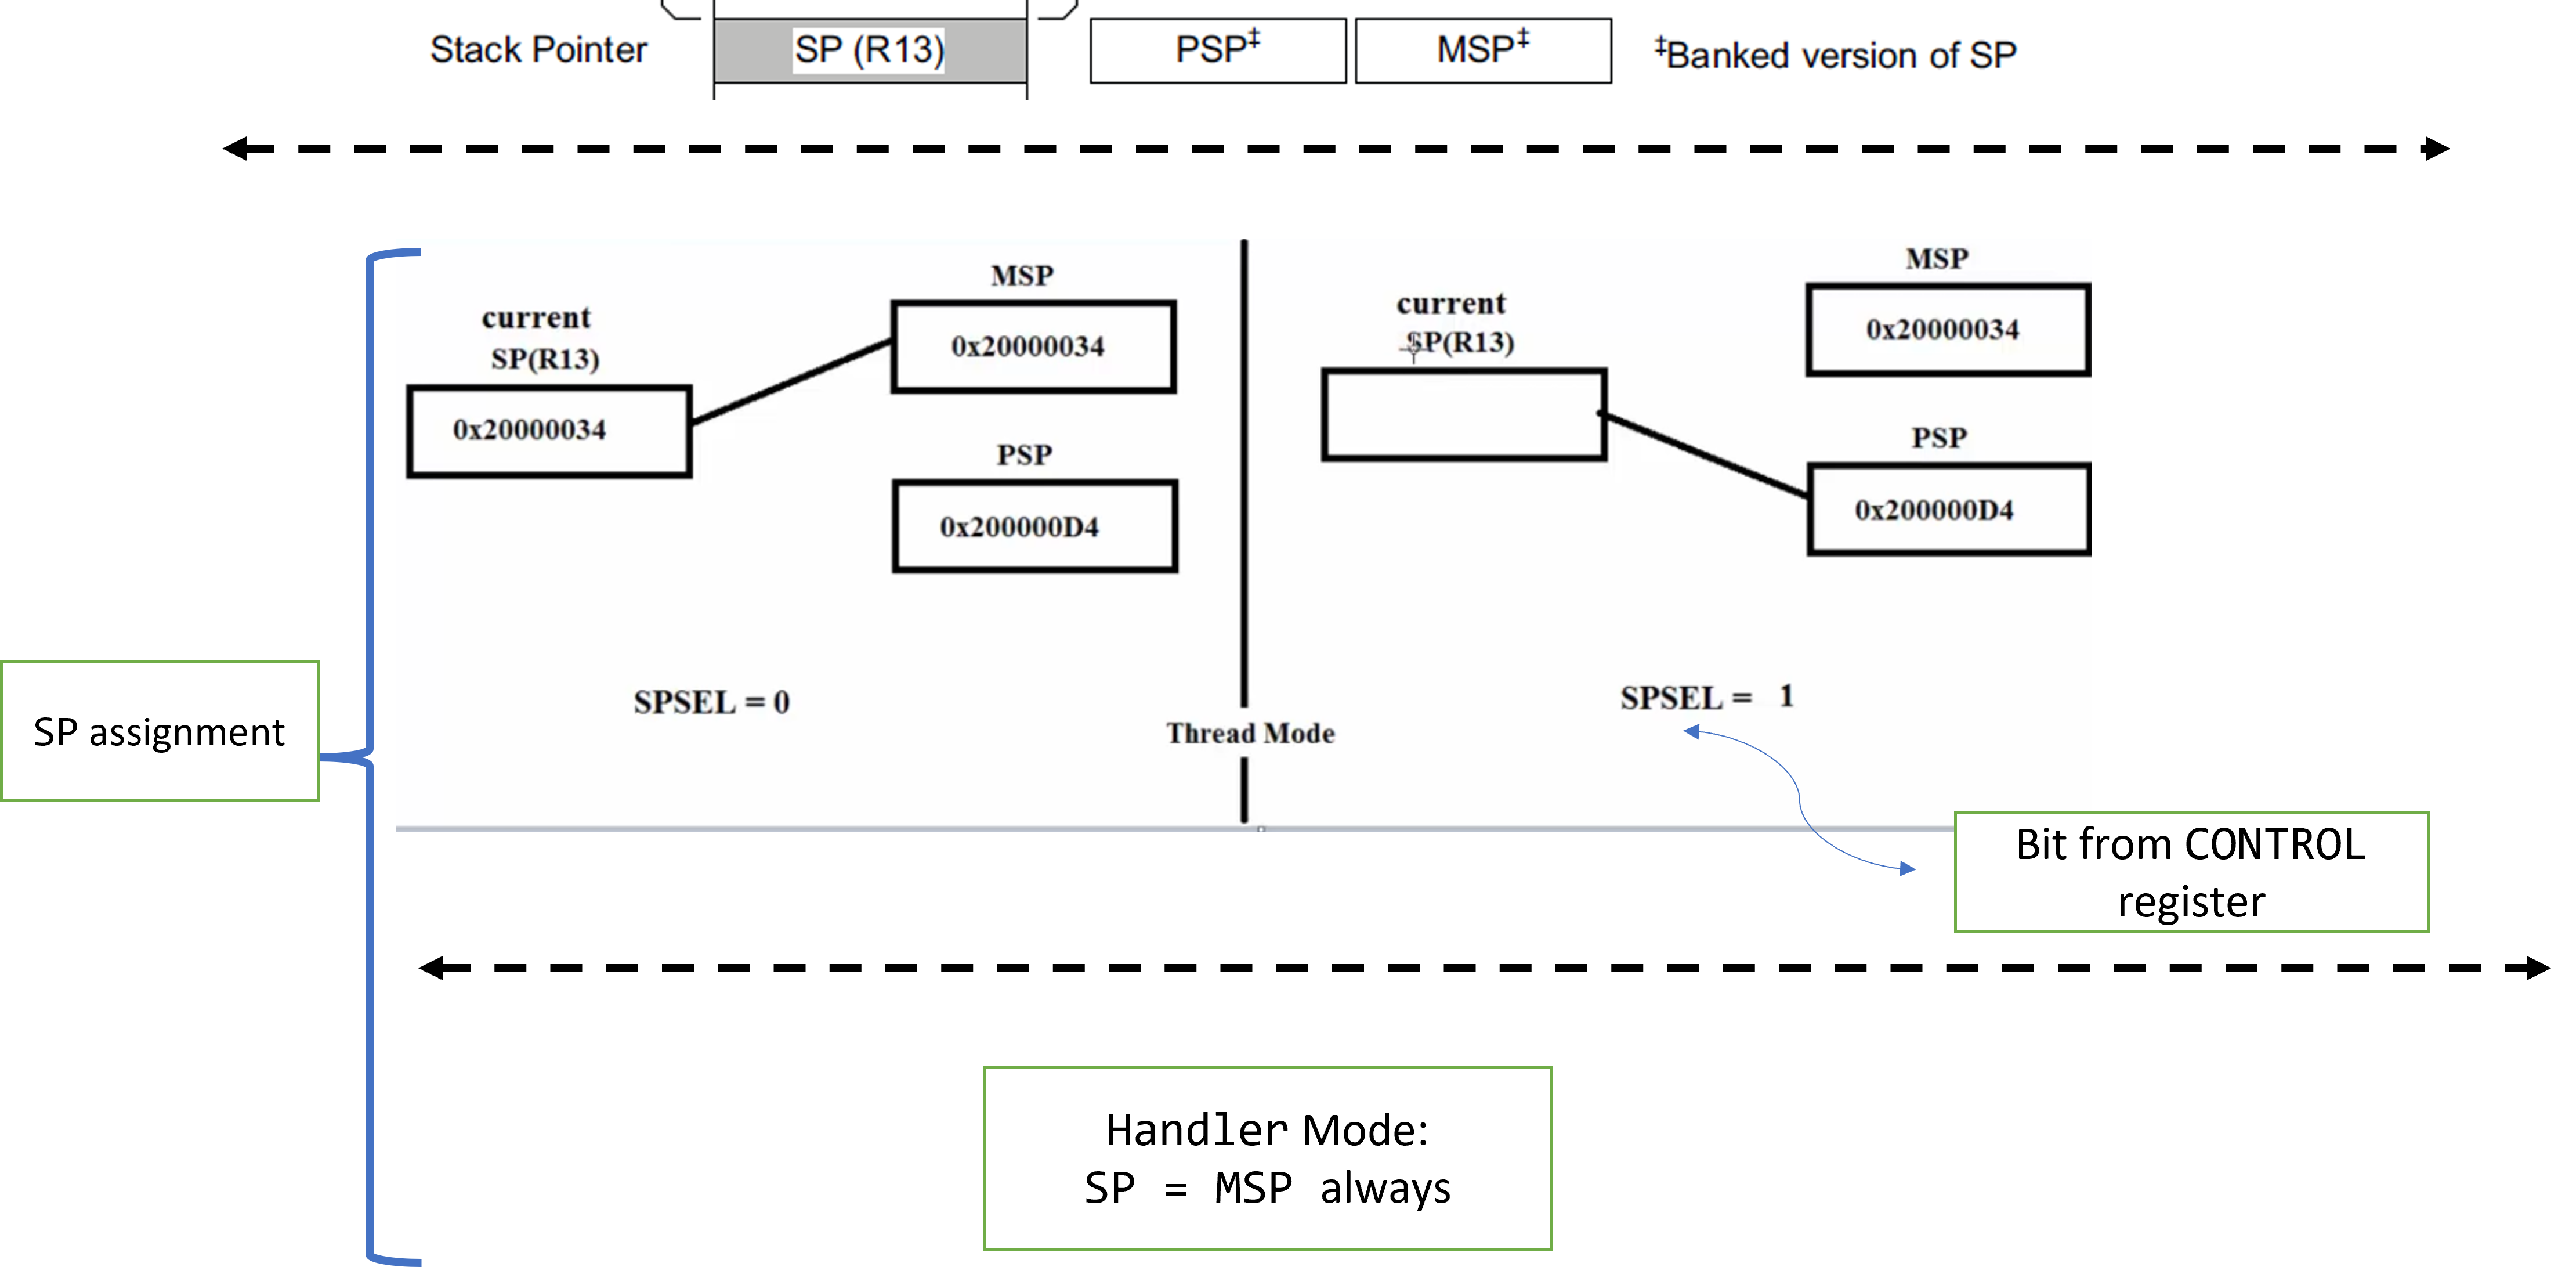
\includegraphics[scale=0.5]{Figures/ARM_Cortex/bank_stack}
\caption{Stack Pointer assignment in thread and handler mode}
\label{fig:ARM_Cortex:bank_stack}
\end{figure}

\begin{itemize}
    \item Initially after reset, \verb|SP| read the content of \verb|MSP|. We can change it to \verb|PSP| by changing the bit value of \verb|SPSEL| from the \verb|CONTROL| register.

    \item In handler mode, \verb|SP = MSP| always
\end{itemize}

\end{itemize}

\subsection{Stack Exercise}

\todo{Stack Ex} \underline{\textit{Stack Ex}:} \textit{Implement a code where we change the SP to MSP. To do it maybe later. See section 10 video 43 and 44.}


\subsection{Function Call for Arm Architecture}

When calling a function, Arm uses a procedure called AAPCS. This procedure is mainly used when writing routines in assembly. As an example, \autoref{fig:ARM_Cortex:function_calling_example_arm} shows an example of this standard, when we have some function calling.

\begin{figure}[h]
\centering
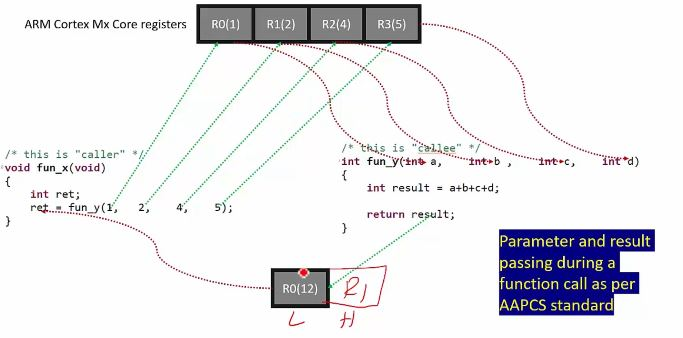
\includegraphics[scale=0.7]{Figures/ARM_Cortex/function_calling_example_arm}
\caption{Stack Pointer assignment in thread and handler mode}
\label{fig:ARM_Cortex:function_calling_example_arm}
\end{figure}

\begin{itemize}
    \item The caller responsibility is to copy the data to the registers (\verb|R0,R1|,till \verb|R3|)

    \begin{itemize}
        \item If more the 4 arguments is used, then we use the stack to store these arguments
    \end{itemize}


    \item  Then the callee copy from the those registers the value to their local variable

    \item  The result is always stored in \verb|R0|, and if we need more then 32 bits, we use \verb|R1| where higher bits are stored.
    
\end{itemize}


\subsection{Stack during Exception and Interrupt}

When calling some function, the AAPCS protocol will be followed. In a big picture, each of caller and the callee has some responsibilities. However, when we have some exception, \tbi{there is no caller} (in other words no AAPCS protocol to apply), because exception and interrupts can be called any time (they are asynchronous in nature), and they are called the processor hardware. At this phase, all the correspondent registers will be saved in the stack frame by the processor.

\newpage

\section{Exceptions}
\label{Sec:Exceptions}

Now we present the concepts of exceptions in a processor. \autoref{fig:ARM_Cortex:exception_def_type} contains definitions and their types.


\begin{figure}[h]
\centering
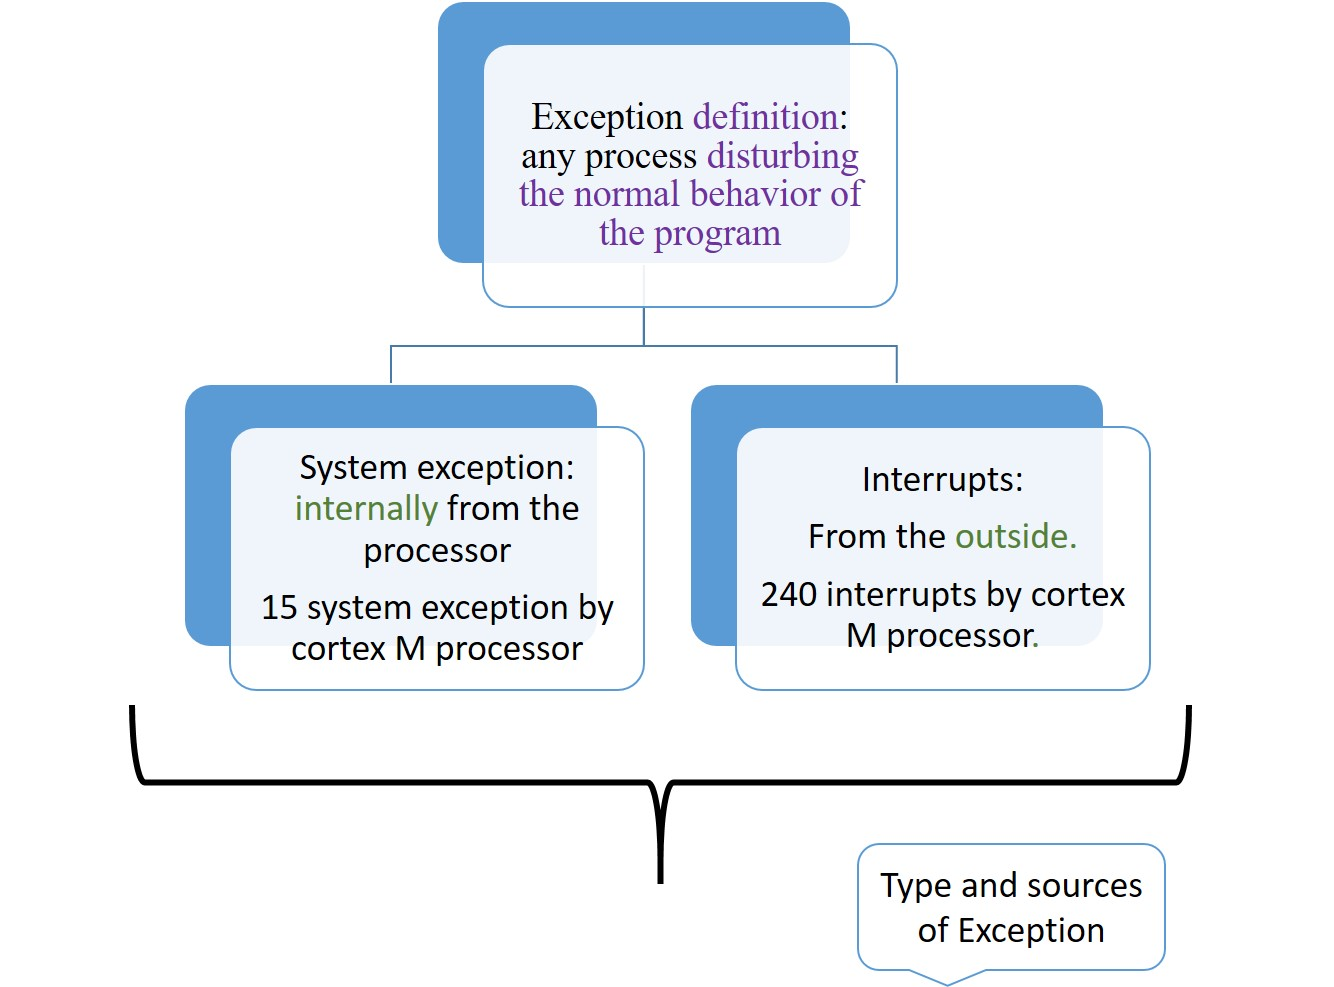
\includegraphics[scale=0.7]{Figures/ARM_Cortex/exception_def_type}
\caption{Exceptions: definition and type}
\label{fig:ARM_Cortex:exception_def_type}
\end{figure}

\begin{itemize}

\item Exception is any type of process which break the normal flow of a code

\item It can comes from inside the processor or outside the processor

\end{itemize}

\subsection{System Exception}

For arm cortex m4, we can see the different system exception in generic user guide, section 2.3 named Exception model.\\

The m4 cortex has as we said earlier (in \autoref{fig:ARM_Cortex:exception_def_type}) has 15 system exception, all illustrated in table 2-16

In general, what we can retain from reading the table and the description, that each exception is triggered by some specific event. Example:

\begin{itemize}

\item UsageFault if we try to divide by 0

\end{itemize}

\underline{Note:} read todo note later, to see why there is not enough content or info

\newpage
\underline{\textit{\textbf{System Exceptions}}:}
 \todo{System Exceptions}

\begin{itemize}

\item \textit{System Exception is in video 48 of the course}

\item \textit{There were allot of theory and no practice about system exceptions, so for now I didn't write any, as infor as simply stated in the manual}

\item \textit{hardFault exception is encountered in the T bit banding excercice}

	\begin{itemize}
	\item \textit{So maybe to do this later}
	\end{itemize}

\item \textit{Maybe after completing the course, to re-write this section later}

\end{itemize}


\newpage
\section{System Exception Vector Address}

System Exception can be found in the reference manual, in what is called a \tbi{vector table} (table 62 page 357).

\todo{Vector Table} \underline{\textit{Vector Table}:}

\begin{itemize}

\item \textit{To see later what is that vector table, and the difference between memory map and the vector table}

\item \textit{In the lectures, I don't remember explaining such kind of tables}

\end{itemize} 

\newpage
\section{System Exceptions Control Registers}

In this section we explore processor registors responsible for the system exceptions (exceptions that come from inside the processor).\\

The arm cortex processor comes with different peripherals, as show in \autoref{fig:ARM_Cortex:processor_peripherals}, where each peripheral comes with its own register set to control a peripheral.

\begin{figure}[h]
\centering
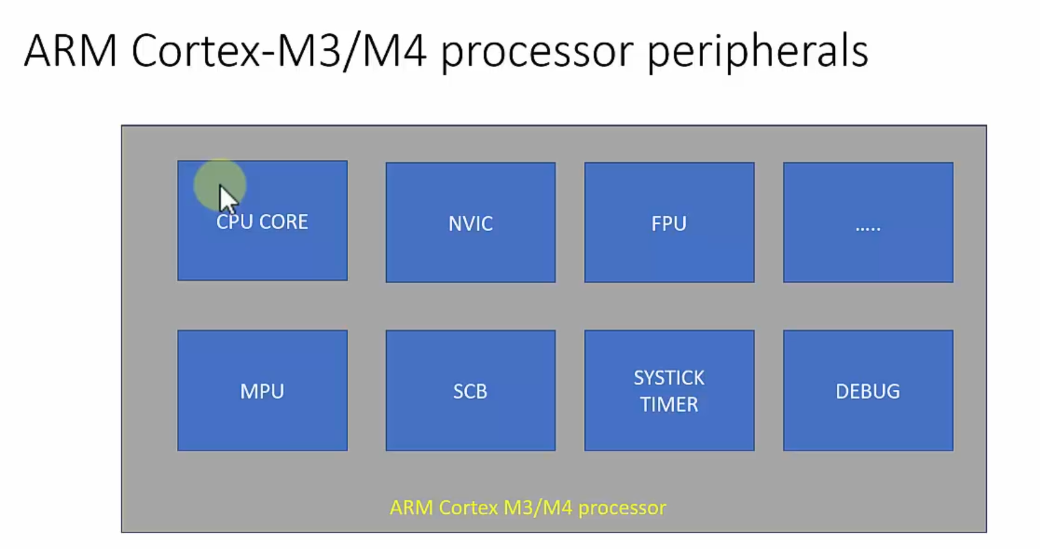
\includegraphics[scale=0.4]{Figures/ARM_Cortex/processor_peripherals}
\caption{Arm cortex Peripherals}
\label{fig:ARM_Cortex:processor_peripherals}
\end{figure}

\begin{itemize}

\item See section 1.1.14 in the generic user guide for peripheral descriptions.

\end{itemize}

\newpage
These peripherals can be accessed via the PPB (private peripheral bus), where its addresse map is shown in \autoref{fig:ARM_Cortex:ppb_addresse_map}.

\begin{figure}[h]
\centering
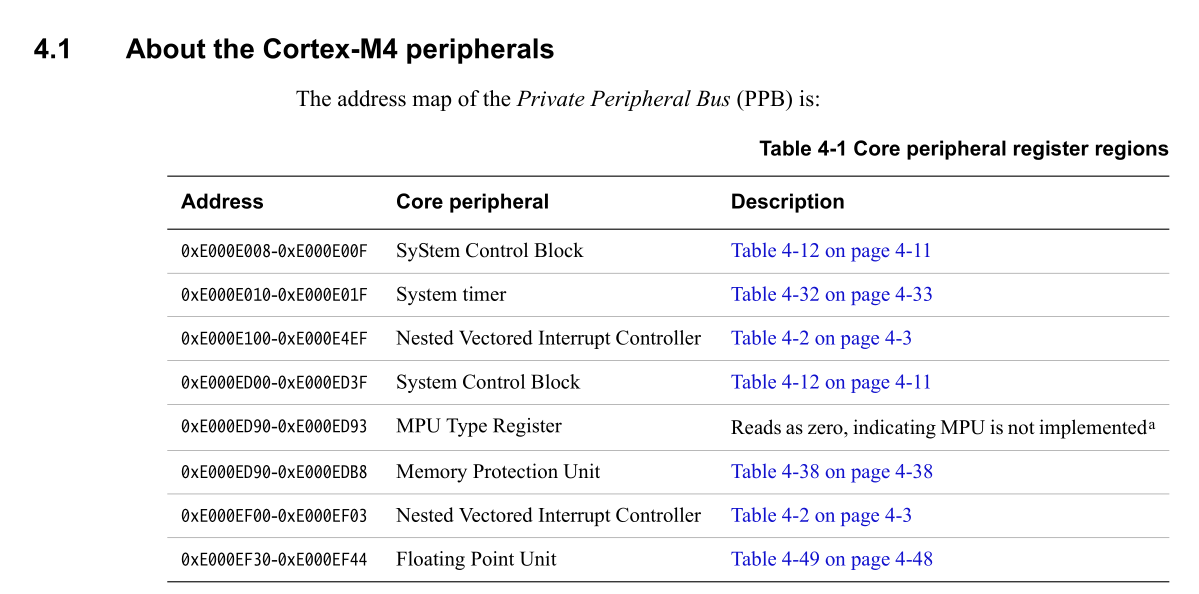
\includegraphics[scale=0.4,frame]{Figures/ARM_Cortex/ppb_addresse_map}
\caption{PPB Adresse map}
\label{fig:ARM_Cortex:ppb_addresse_map}
\end{figure}

\begin{itemize}

\item The table in \autoref{fig:ARM_Cortex:ppb_addresse_map} can be found in the generic user guide of the arm cortex, page 218.

\end{itemize}

\newpage
\section{NVIC}

NVIC stands for nested vector interrupt controller, and its one of the arm-cortex peripherals.\\

The NVIC is used to control the 240 interrupts external to the processor. In other words, it controls the traffic of the interrupts coming to the arm processor.\\

\underline{Note:} 

\begin{itemize}

\item recall that external means that these interupts are not generated by the processor.

\item for interrupts, the NVIC hardware is responsible to control the traffic of the interrupt

\item for the system exceptions (interrupts generated from inside the processor), the system control block (see \autoref{fig:ARM_Cortex:ppb_addresse_map}, where its mentioned its addresse space) is the entity responsible

\end{itemize}


\subsection{NVIC doc}

The NVIC detailed description can be found in the arm generic user guide, section 4.2. 

\subsection{Interrupt sources}
\label{sub:Interrupt_sources}

Now a question arise: what are exactly these 240 interrupts ?\\

Well the answer to that question can't be found in the arm generic user guide, but rather in the reference manual of the microcontroller (table 62 page 357).\\

In stm32f407 discovery board, among the 240 interrupts provided by arm, stm (the microcontroller vendor) has implemented 82 interrupts.

We can see them in table 62, spanning from 0 $\rightarrow$ 81.\\

So in other words, the microntroller vendor is responsible of the external interrupt. 
These interrupts are coming from the micrcontroller peripherals, such as GPIO, SPI, timers,$\cdots$. 

\subsection{Generic design}
\label{sub:interrupt_generic_design}

To recap,  figure \autoref{fig:interrupts:design_concept} present a generic design.

\begin{figure}[h]
\centering
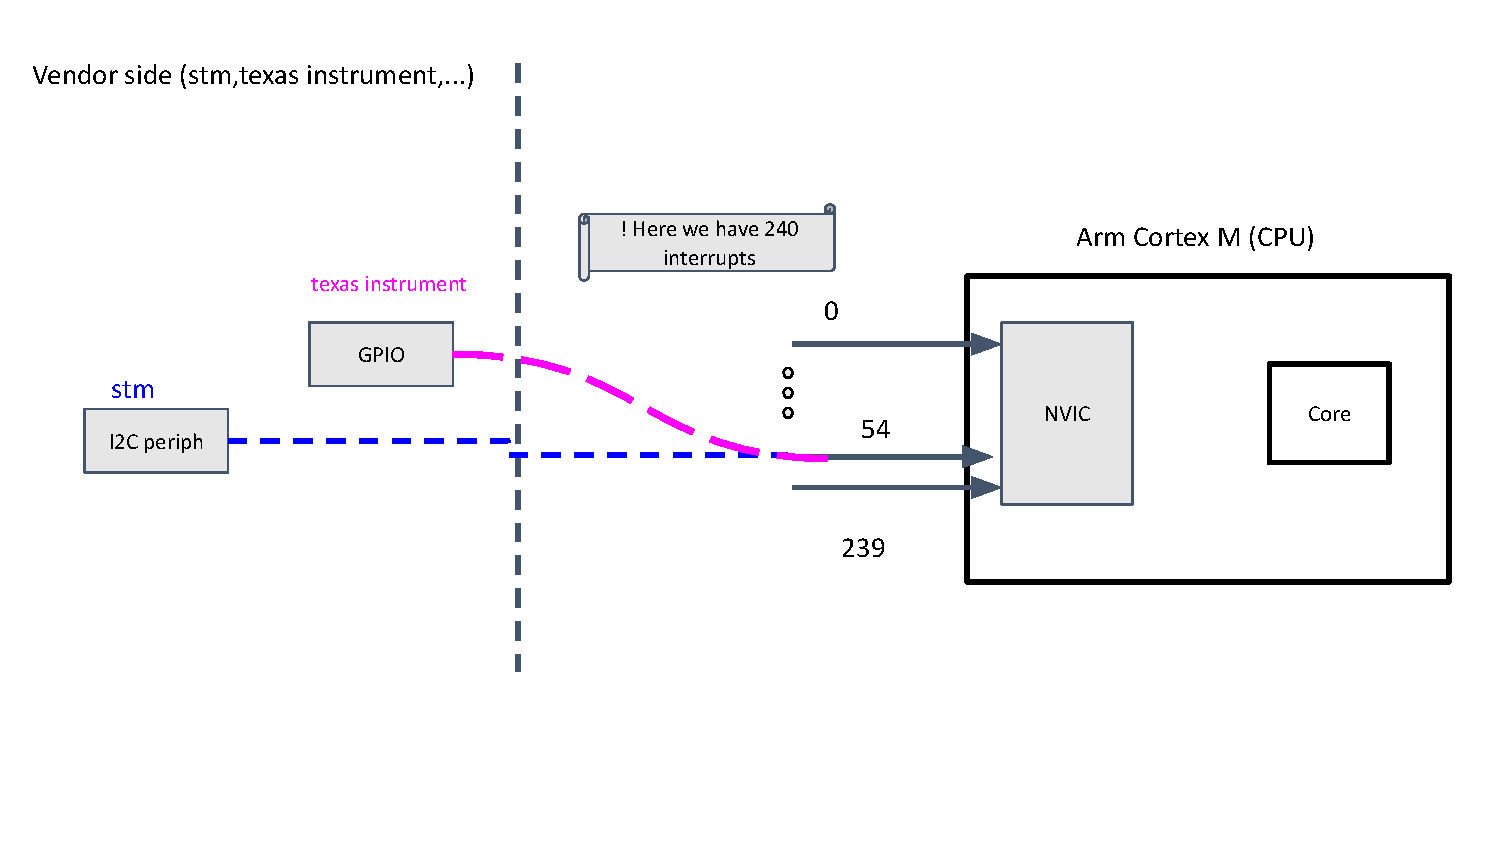
\includegraphics[scale=0.7,frame]{Figures/interrupts/design_concept}
\caption{PPB Adresse map}
\label{fig:interrupts:design_concept}
\end{figure}


\begin{itemize}

\item In the right hand side, we have the arm processor

	\begin{itemize}
	\item The NVIC peripheral is shown along with its 240 lines
	
 
	\end{itemize}

\item The lines of the NVIC takes input form the peripheral of the micrcontroller

\item Each micrcontrtoller vendor has the choice of design to select which peripheral uses whihc line to send an interrupt signal

\item Example: st for example, uses line 0 for the watchdog pereipheral

	\begin{itemize}
	\item since watchdog uses line 0, its number is called IRQ0
	\end{itemize}

\item 2 vendors (such as stm and texas instrument for example), can use the same IRQ number, but to take interrupts from 2 different peripherals

	\begin{itemize}
	\item We have an example for IRQ54 in \autoref{fig:interrupts:design_concept}, where the line is used by 2 different peripheral for each vendor
\end{itemize}	 

\end{itemize}

\newpage
\subsection{NVIC Registers}

To explore the NVIC registers, we open the arm-generic user guide, section 4.2. This section describe all registers, and also there is table Table 4-2, which contains a register summary.\\

Now let's begin the sruvey.\\

\underline{Interrupt Set-enable Registers:}

\begin{itemize}

\item there are 8 registers (from 0 $\rightarrow$ 7) to handle the 240 interrupt

\item If we take for example \verb|NVIC_ISER0|, we can set 32 interrupts, since this register contains 32 bit.

\item \verb|NVIC_ISER0| can be \tbi{used only to enable interrupt} $\leftrightarrow$ we can't disable an interrupt via this register

\end{itemize}

\underline{Interrupt Clear-enable Registers:}

\begin{itemize}

\item also we have 8 registers to cover the 240 interrupts

\item this register is used to disable an interrupt, but setting some bit to 1 (again 0 has no effect)

\end{itemize}

\underline{Interrupt Active Bit Registers:}

\begin{itemize}

\item Also 8 registers we have

\item Used to see which interrupt is active (executed by the processor)

\end{itemize}

\underline{\textit{Pending}:} \todo{Pending} 

\begin{itemize}

\item \textit{There is what is called Interrupt Set-pending Registers and Interrupt Clear-pending Registers}

\item \textit{The concept of pending I didn't understood it yet, since we didn't work with some example or code}

\item \textit{See video 52 when he describe the pending, and the priority concept related to it}

	\begin{itemize}
	\item \textit{Again, the concept of priority wasn't explain also}
	\end{itemize}

\end{itemize}


\newpage
\section{Peripheral Interrupt Exercice}

Now we will do some coding exercice, about the interrupt generated by some peripheral of the micrcontroller. The description is shown in \autoref{fig:ARM_Cortex:periph_interrupt_coding}.

\begin{figure}[h]
\centering
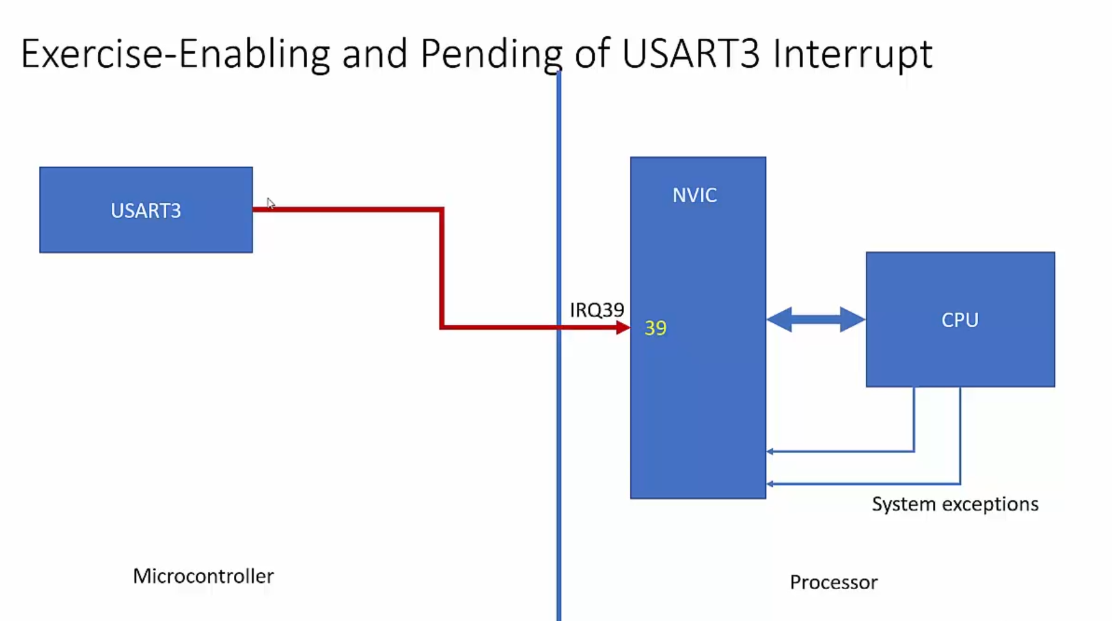
\includegraphics[scale=0.4,frame]{Figures/ARM_Cortex/periph_interrupt_coding}
\caption{Interrupt by USART Periphral}
\label{fig:ARM_Cortex:periph_interrupt_coding}
\end{figure}

\begin{itemize}

\item The peripheral is USART3

\item If we look to the reference manual (table 62), the USART3 peripheral has and IRQ number equal to 39

\end{itemize}

\subsection{Interrupt programing steps}

Before diving into the code, let's state some general steps for interrupt programming

\begin{enumerate}

\item Identify what is the IRQ number for the particular peripheral we are working with

	\begin{itemize}
	\item Recall that IRQ number are \text{vendor specific} $\leftrightarrow$ stm has different attribution for IRQ number the texas instrument for example
	\end{itemize}

\item Enabling the IRQ via registers of the processor (that is the Arm cortex registers, document in the generic user guide)

	\begin{enumerate}
	\item we can also the configure the \tbi{priority}, which is optional
	
	\item By default, and interrupt has the higher priority, equal to 0
	
	\item We will see later interrupt prorities in another sections
	
	\end{enumerate}

\item 

\end{enumerate}

\todo{MCU Periph Interrupts} \underline{\textit{MCU Periph Interrupts}:}

\begin{itemize}

\item \textit{To review later the paragraph above}

\item \textit{See video 53 at 5:31}

\end{itemize} 


In \autoref{fig:interrupts:diagram_interrupt_execution}, we have a diagrame of how an interrupt will be executed

\begin{figure}[h]
\centering
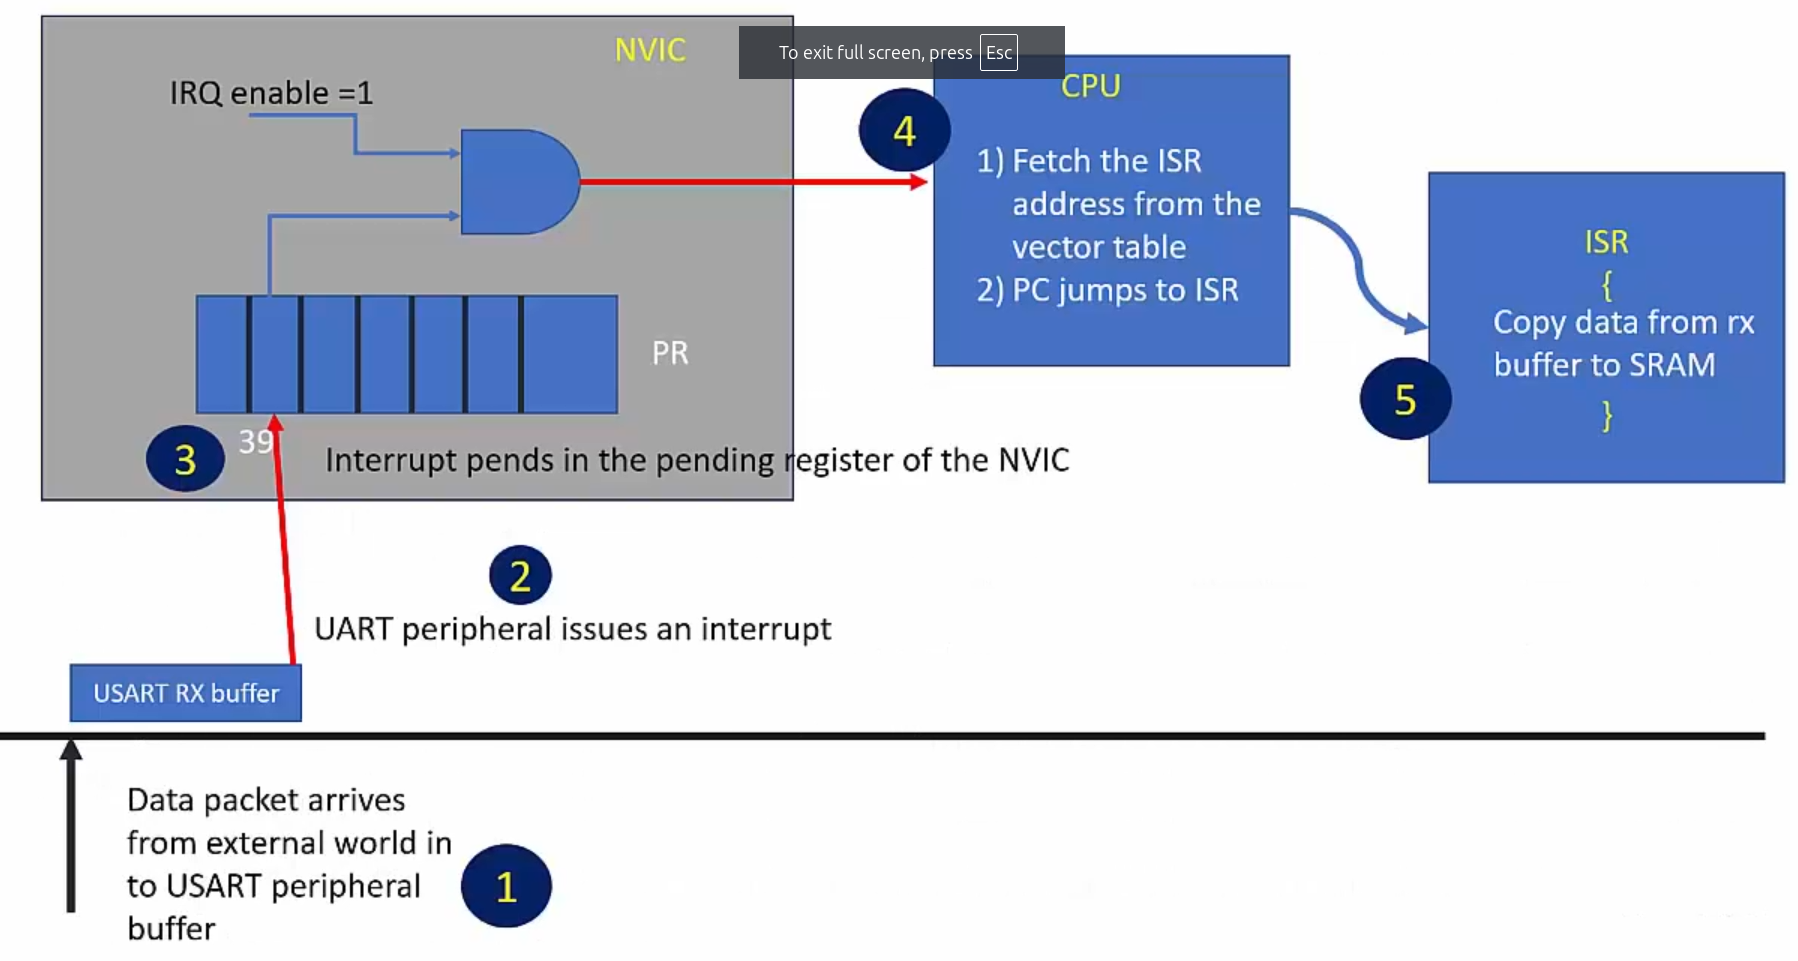
\includegraphics[scale=0.2,frame]{Figures/interrupts/diagram_interrupt_execution}
\caption{Interrupt by USART Periphral}
\label{fig:interrupts:diagram_interrupt_execution}
\end{figure}

\begin{itemize}

\item Interrupt are \tbi{triggered by some events always}

	\begin{itemize}
	\item In the case of USART, is the arrival of a packet in the Rx buffer (step 1)
	\end{itemize}
	
\item Once the USART3 Rx buffer is full, it triggers an interrupt on the IRQ line, and make the line high or low (step 2)

Until now, step 1 and 2 are from the peripheral side

\item When the interrupt is issued, it will set the pending state in the pending register of the NVIC (step 3)

	\begin{itemize}
	\item now we start processor side sinc we are in the NVIC
	\end{itemize}

\item If the IRQ is enabled, the NVIC will allow the interrupt to be executed and send it to the processor (the CPU) $\leftrightarrow$ the NVIC interrupt the CPU (step 4)

\item  When the interrupt is accepted by the CPU, the CPU will

	\begin{itemize}
	\item fetches the ISR address for that IRQ number in the vector table
	
	\item the processor (program counter) jumps to the ISR
	\end{itemize}

\item In the ISR, we can copy the data from the RX buffer to the memory (the SRAM)

\end{itemize}


\newpage
\section{Summary: Embedded System on Arm Cortex M3/M4}
\label{Chap:Arm_cortex:Summary}

\begin{itemize}

\item Motivation behind ARM cortex

\begin{itemize}
    
    \item ARM cortex processor are used in most microcontoller manufacturing because of its minimal cost (save money),minimal power,minimal silicon area


    \item It is based on 32 bit architecture which can boost computational power, and has same price as traditional 8 and 16 bit processors

    \item It can be customizable to include different units (DSP units, memory protection units,floating point units,$\cdots$), depending on the target application 

    \item RTOS friendly

    \item Instruction set is rich and memory efficient
    
    \todo{Instruction set} \underline{\textit{Instruction set:}}  \textit{to be reviewed later why it is efficient}.

    \textit{The instruction set concept maybe I saw it in previous chapter, to be seen later.}

     \end{itemize}   

\item Key concepts

    \begin{itemize}
        \item A processor is nothing but a processor core + surrounding peripheral.

        \item A microcontroller =  a processor + some other peripheral, connected by many \textit{buses} 

        \item Keep mind that not all vendors uses ARM cortex architecture (some of them use their own CPU architecture in their microcontroller)
        
    \end{itemize}



\item See the assembly of the \verb|C| file:

\begin{enumerate}
    \item Build the project

    \item Right click on the project

    \item \verb|Properties|, a pop window will appear as shown in \autoref{fig:ARM_Cortex:file_location}.


    \begin{figure}[h]
\centering
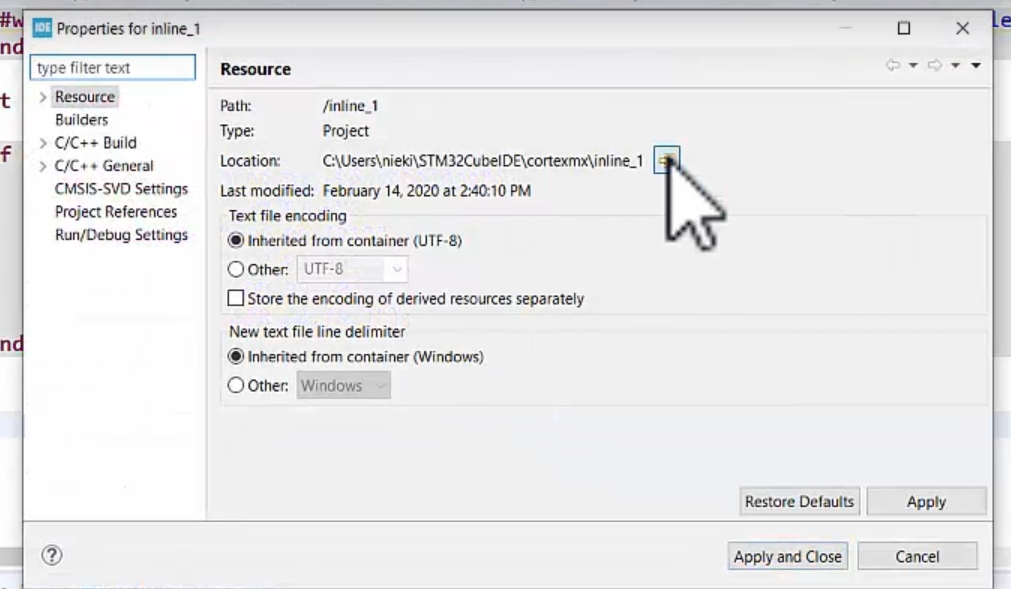
\includegraphics[scale=0.55]{Figures/ARM_Cortex/file_location}
\caption{Go to file location}
\label{fig:ARM_Cortex:file_location}
\end{figure}

It will take us to the project

\item We go inside the project and click on the \verb|Debug| folder

\item We open the file with \verb|.list| extension.

    
\end{enumerate}


\item Variable created in the \verb|C| file are in the stack (so in the RAM)

\item Inline assembly language: used whenever we need to control some registers presented in the core , and can't be accessed by standard \verb|C| code.

For details see \autoref{Sec:inline_assembly}.

\item The reset handler function:

\begin{enumerate}
    \item doing some initialization


    \item Call the \verb|main| function
\end{enumerate}

\item \underline{Design Concept:} we have 2 bus (AHB and APB) because by this way, MCU vendors can put the peripheral which don't require high speed on low performance bus (the APB in our case) and reduce power consumption.

\newpage
\item  Exceptions (\autoref{Sec:Exceptions}):

\begin{figure}[h]
\centering
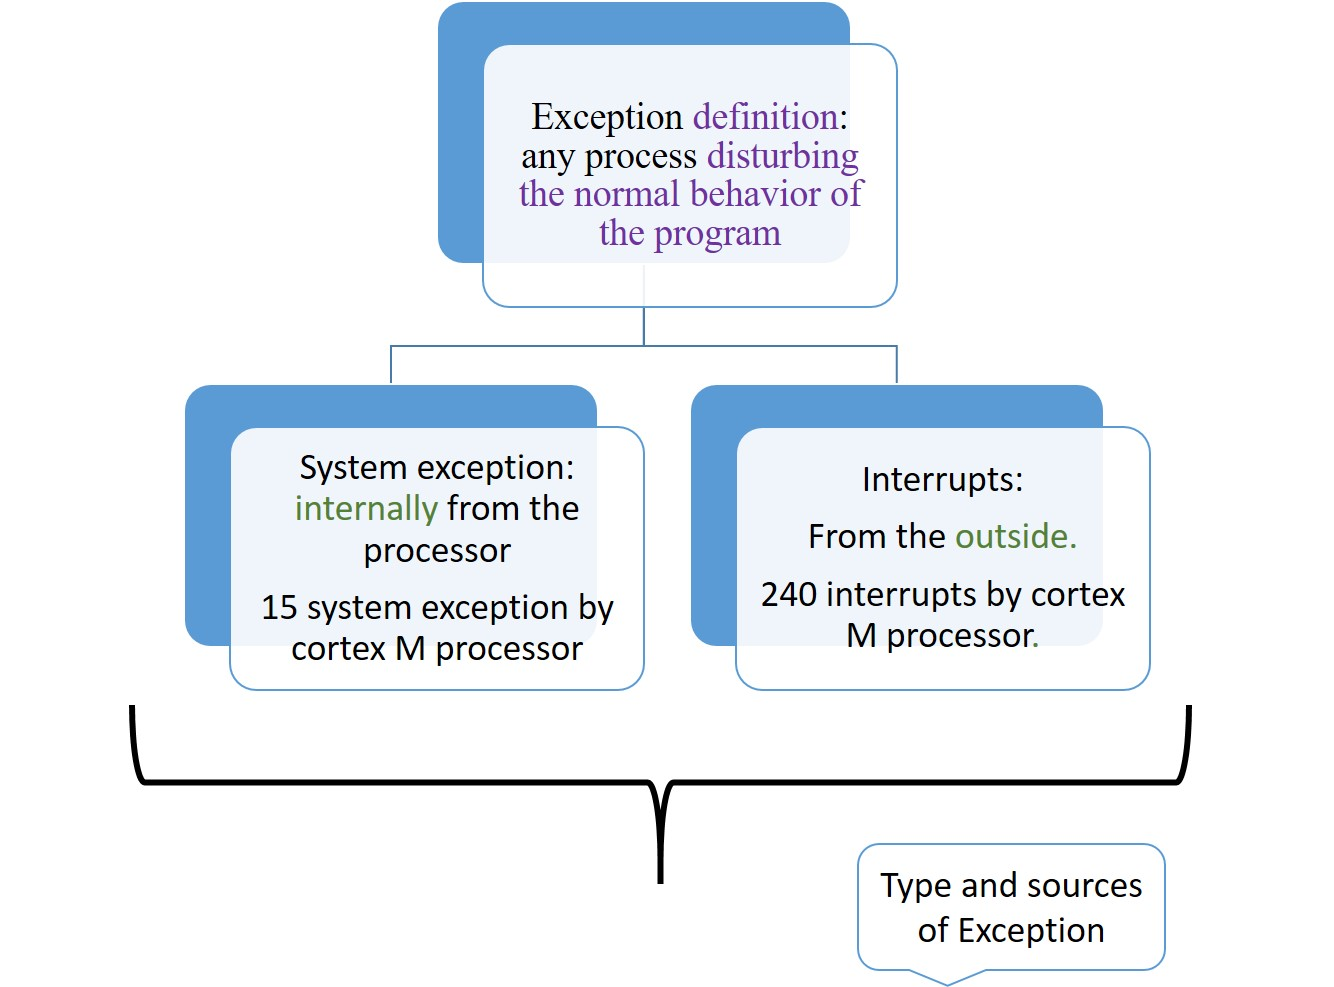
\includegraphics[scale=0.7]{Figures/ARM_Cortex/exception_def_type}
\caption{Exceptions: definition and type}
\label{fig:ARM_Cortex:exception_def_type}
\end{figure}

Keep in mind that exceptions:

	\begin{itemize}
	
	\item break the normal flow of the code
	
	\item their are 2 types: 
	
	\begin{enumerate}
	\item 	\tbi{internal} $\leftrightarrow$ from inside the microcontroller $\leftrightarrow$ called system exceptions	
	
	\item \tbi{external} $\leftrightarrow$ from outside the micrcontroller $\leftrightarrow$ \tbi{interupts}	

	\end{enumerate}		
	
	\end{itemize}


\item Doc for exceptions:

	\begin{itemize}
	\item Generic user guide:
	
		\begin{itemize}
		\item section 2.3: Exceptions Model page 2-21 (34)
		
		\item Arm cortex peripheral chapter: 		
		
		\item the peripherals side of the arm cortex: system control block page 4-11 (227) responsible for system exceptions
		
		\item NVIC page 219 section 4.2, responsible for the interuupt side
		\end{itemize}				
	
	\item Reference Manual:
		
	\begin{itemize}
	\item Vector Table table 62 page 357 	
	\end{itemize}		
	
	\end{itemize}
   
\item Sources of interrupt: see \ref{sub:Interrupt_sources} and \ref{sub:interrupt_generic_design}   
   
\end{itemize}

\newpage
\section{TODO Arm Cortex}

\begin{itemize} % start imtemize initial

\item An idea: I might split up this chapter based on Zhu book

	\begin{itemize}
	\item But $\mathrm{1}^\mathrm{st}$ I need to review later sections talking about the arm cortex in general in my report
	
	\item Combine this with reading in Zhu book
	
	\item Chapter 3 is a good starting point 	
	
	\end{itemize}


\item Search about different type of Arm cortex family

	\begin{itemize}
	\item difference between M0,M4,M7,...
	\end{itemize}

\item To redo later all the sections related to processor registers

	\begin{itemize}
	\item It was too much theory
	
	\item I will search for some applications, or a goal later about these ideas 
	\end{itemize}


\item To see later what is vector table, and its relation with exception addresses in the memory map of the microcontroller

	\begin{itemize}
	\item I don't recall or note in my report a definition of this kind of tables
	\end{itemize}

\end{itemize} % End itemize initial


% ============== END Chapter ==============

